\documentclass[../thesis-main.tex]{subfiles}

\begin{document}

\chapter{Literature Review}
\label{ch:litreview}

\begin{aquote}{\emph{Hamlet}, Act 1, Scene 5}
  {\fontencoding{T1}\fontfamily{pzc}\selectfont
   There are more things in heaven and earth, Horatio,\\
   Than are dreamt of in your philosophy.
  }
\end{aquote}
\rule{\linewidth}{0.25mm}

  \begin{quote}
   \emph{In this section, the relevant background information is given. This starts with a brief outline of the function and structure of the heart, ranging from the high order organisation of the heart into functional compartments, down to the cellular level. Further details are then given on the physiological aspects of some of the subcellular components of cardiac tissue. The evolution of computational models to describe the electrical activity of the heart is charted briefly, with special attention given to models specifically used in this thesis. Variation is then described, both in experimental and physiological measurements, and how this variation has been addressed in computational models. Then the pathological condition of isch\ae{}mia will be described, and the computational efforts to model this outlined.}
  \end{quote}


 \section{Cardiac Physiology}
 \label{sec:physiology}
 At the most general level, the heart serves as a pump to transport blood around the body to deliver nutrients and remove waste products. It does this by rhythmic, organised contraction---the rate of this contraction varies depending on species, age, condition of the heart and the activity being undertaken by the organism.
 
 \subsection{Structure of the Mammalian Heart}
 \label{subsec:heart-structure}
 \begin{figure}
  \centering
  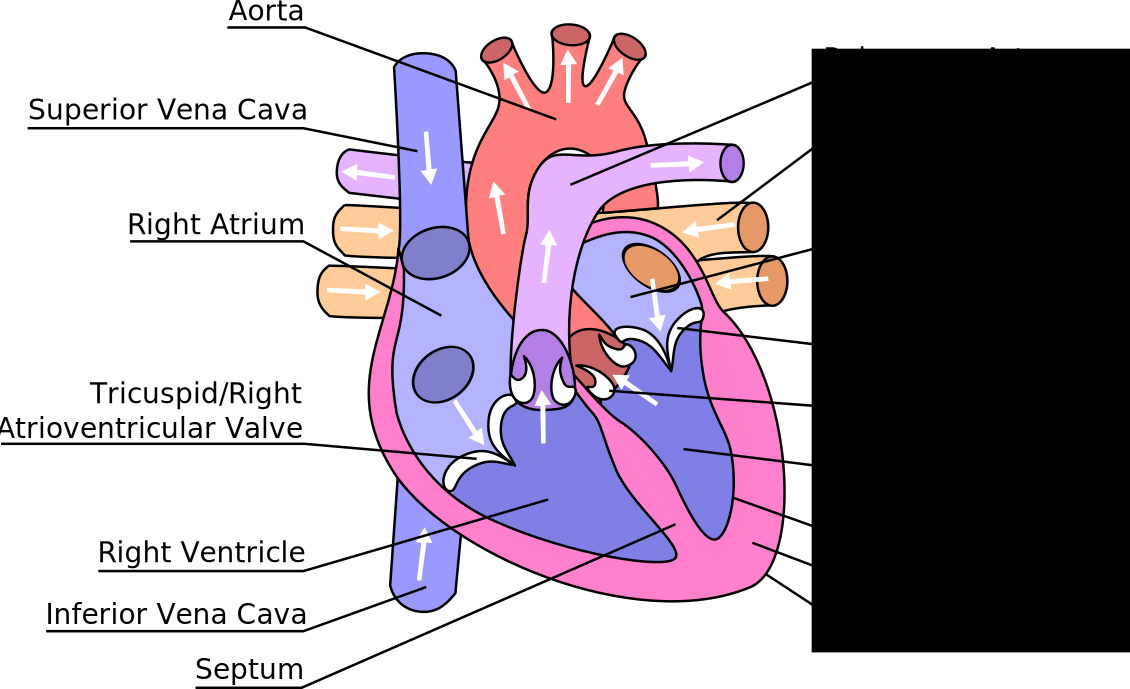
\includegraphics[width=0.75\textwidth]{heart_labels}
  \caption[Structure of the mammalian heart]{Diagram of the longitudinal cross-section of a mammalian heart. The direction of blood flow is shown by white arrows, and all major structural components are labelled.}
  \label{fig:heart-structure}
 \end{figure}
 Fig.~\ref{fig:heart-structure} shows the anatomical structure of the mammalian heart---while the size obviously varies widely between mammals, the overall architecture remains constant. It is split into two halves, left and right, by a muscular wall called the \emph{septum}, and then further subdivided into two chambers, the larger, lower chamber being a \emph{ventricle}, and the smaller, upper chamber called an \emph{atrium}.
 
 The passage of blood through the heart follows thus: firstly, deoxygenated blood from the body enters the heart via the superior and inferior/posterior \emph{vena cava}, with superior and inferior representing whether the blood comes from the upper or lower half of the body respectively. Via this channel, it enters the \emph{right atrium}. Passing through the \emph{tricuspid valve} (also known as the right atrioventricular valve), the blood enters the \emph{right ventricle}, where it is then pumped via the \emph{pulmonary artery} to the lungs, where it is oxygenated. The blood returns to the heart via the \emph{pulmonary vein}, entering the \emph{left atrium}, before moving through the \emph{mitral valve} (also known as the left atrioventricular valve) into the \emph{left ventricle}. The blood is then pumped via the \emph{aorta} to the rest of the body. The valves in the heart serve to ensure the flow of blood is always in the correct direction.
 
 The walls of the heart are mostly composed of muscular tissue known as \emph{myocardium}. The thickness of the myocardium is not constant throughout the heart, being thickest in the left ventricle, which requires the greatest force of contraction to pump the blood from the heart to the rest of the body. The myocardium can be split into three different regimes, as labelled in italics in Fig.~\ref{fig:heart-structure}: the \emph{epicardium} is the outermost layer of the myocardium, the \emph{midmyocardium} is the middle layer, and the \emph{endocardium} is the innermost layer. The cells composing these different layers possess different electrophysiological properties; the differences, and the consequences, will be expanded upon in \S\ref{subsec:electro-prop}.
 
 \begin{figure}
  \centering
  \begin{subfigure}[b]{0.45\textwidth}
   \centering
   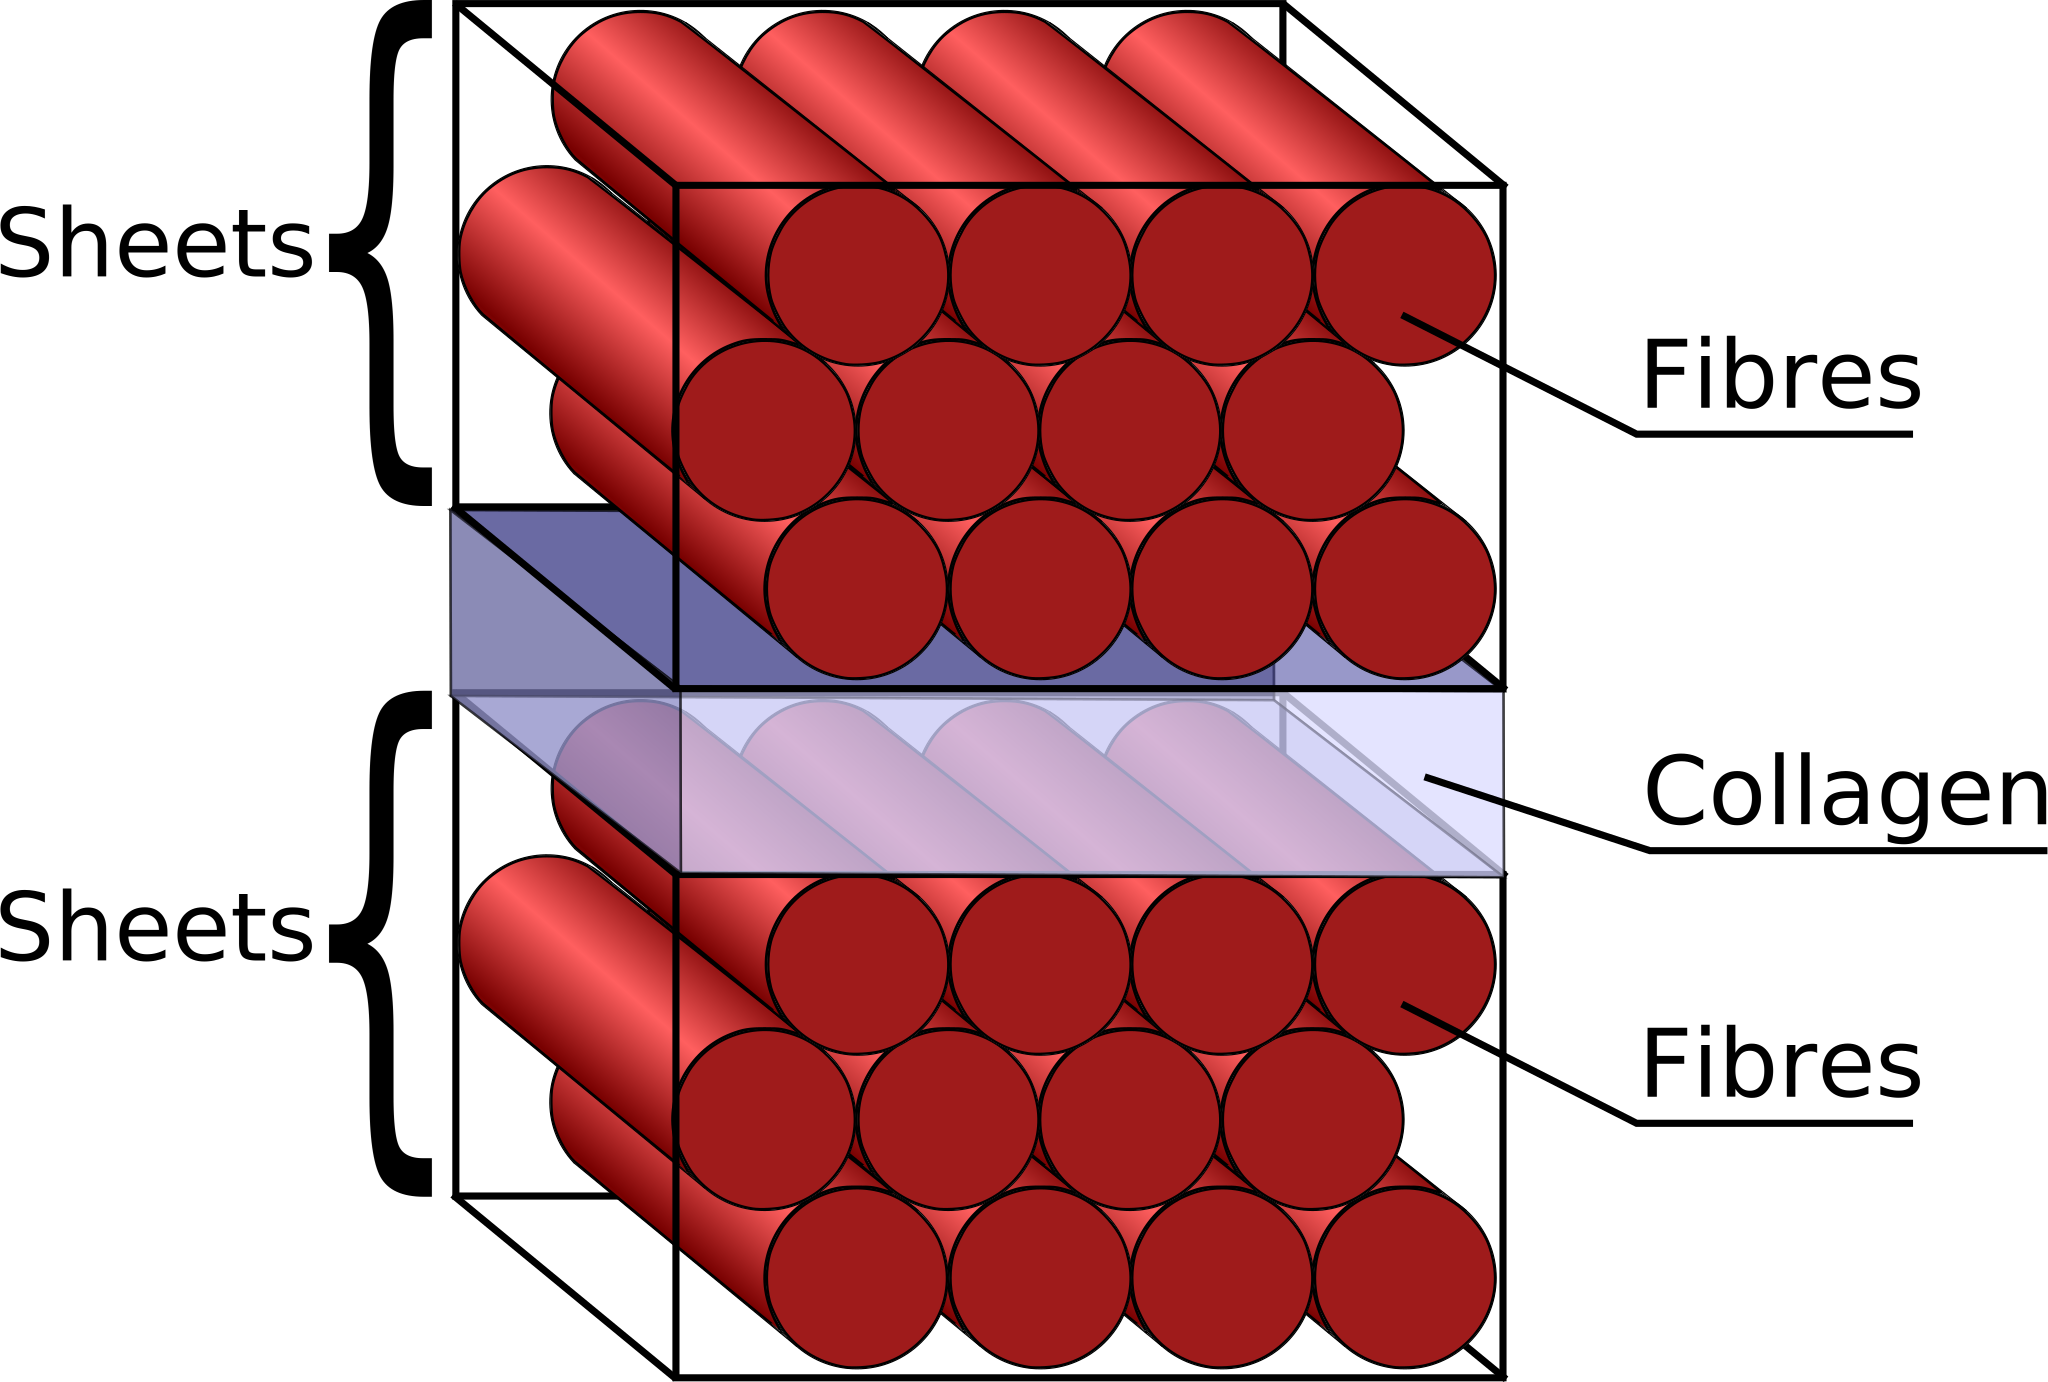
\includegraphics[width=\textwidth]{myocytes}
   \caption{Schematic}
   \label{subfig:myocyte-diagram}
  \end{subfigure}
  \begin{subfigure}[b]{0.45\textwidth}
   \centering
   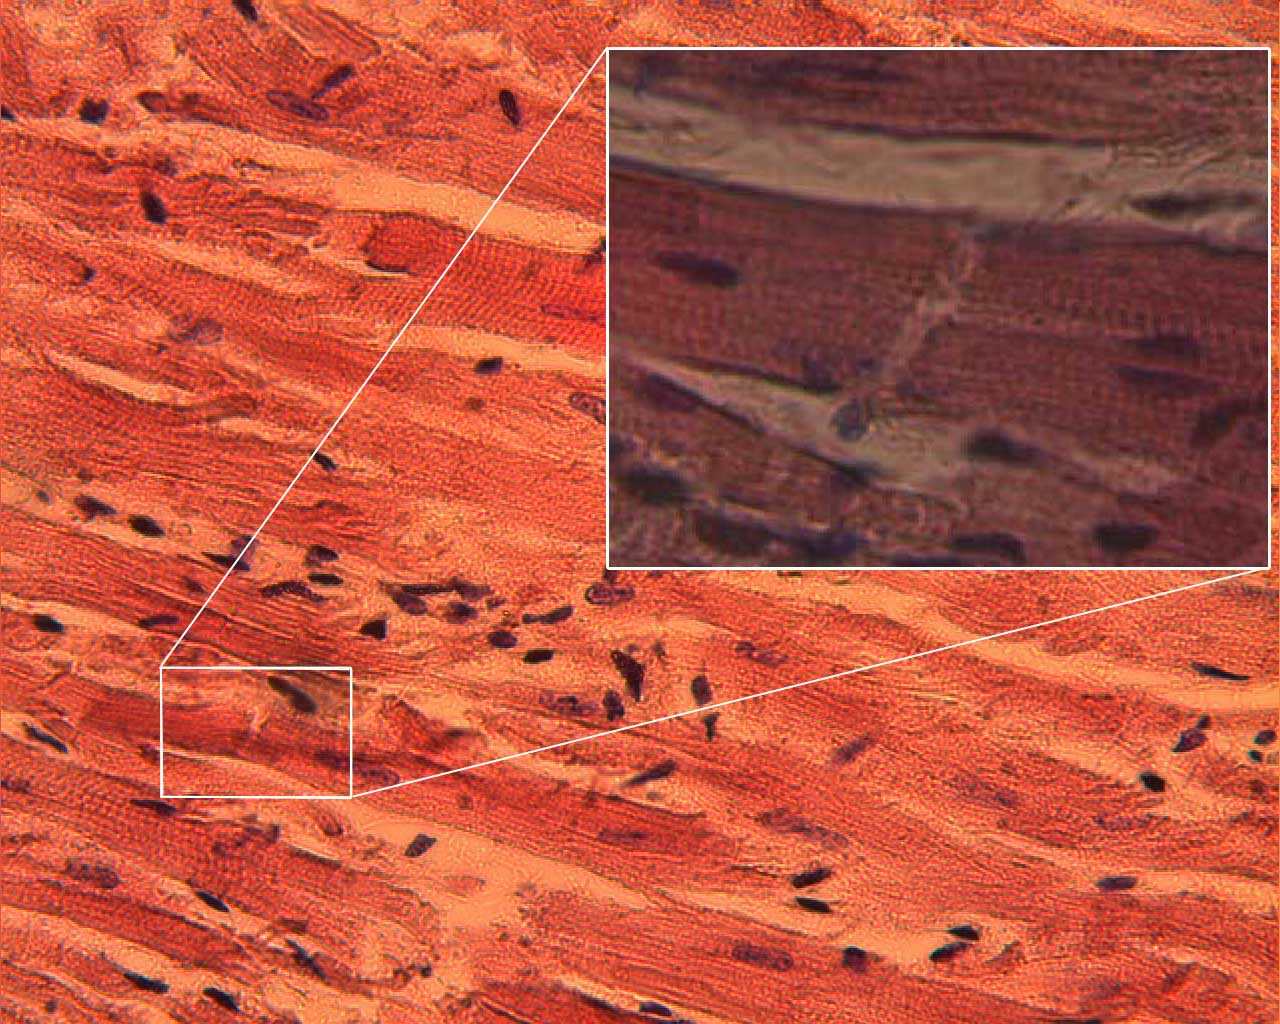
\includegraphics[width=\textwidth]{myocyte-image}
   \caption{Image}
   \label{subfig:myocyte-image}
  \end{subfigure}
  \caption[Structure of myocardial sheets and fibres]{(\ref{subfig:myocyte-diagram}) Schematic of the structure of myocardial sheets and fibres. (\ref{subfig:myocyte-image}) Image of cardiomyocytes demonstrating the interconnected nature of the individual myocytes into fibres \citep{Girod2006}.}
  \label{fig:myocyte-structure}
 \end{figure}
 
 The structure within the myocardium is shown in Fig.~\ref{subfig:myocyte-diagram}: it is composed of a series of sheets of tissue (usually 4 to 6 cells thick) separated by collagen. The myocytes themselves lie longitudinally in these sheets to form fibres, with myocytes connected to each other by intercalated discs spanning the $100-200\AA$ separation between the cells (as opposed to skeletal muscle, which is composed of multinucleated fibres); this structure is seen in Fig.~\ref{subfig:myocyte-image}. One attribute of these discs is the presence of \emph{gap junctions}, which serve to electrically couple the myocytes by allowing ion flow between neighbouring myocytes. It has been shown the \ca{} ions can crosss the gap junctions in a so-called \emph{calcium wave}, triggering activity in neighbouring cells \citep{Miura1998}. This \ca{}-based `triggered propogated contraction' moves more slowly than the \na{}-dependent action potential (the usual means for conducting the electrical activity through the heart tissue) \citep{Clusin2003}. It should be noted that the cells are electrically coupled by more than just gap junctions, \eg{} ephaptic coupling and \K{} accumulation in the membrane space; for a full review of these coupling methods, see \citet{Sperelakis2002}.
 
 In the ventricles, the gap junction distribution is even between fibre direction and off-direction, with each myocyte being electrically coupled to $\sim11$ neighbouring myocytes \citep{Smaill2013}. This arrangement allows isotropic spread of an AP through the ventricle. In the atria, the gap junctions are preferentially in the fibre direction, meaning the AP spread is far more anisotropic \citep{Saffitz1994}. The arrangement of the myocytes into fibres, and the arrangement of these fibres into sheets, allows for ordered contraction in the fibre direction; the fibrous structure also allows the heart to twist as it contracts, leading to a more efficient pumping mechanism.
 
 The conduction pattern of the heart is key to the effective pumping mechanism---by controlling the sequence of electrical events in the heart, the sequence of conduction is similarly controlled. An outline of the conduction pattern of the heart is shown in Fig.~\ref{fig:conduction-pattern}. The sequence of activation starts amongst a complex of self-excitatory cells at the top of the right atrium, called the \emph{sinoatrial node}. This node is electrically isolated from the atria, save for specialised conduction pathways; this both prevents depression of the self-excitation of the node by the hyperpolarising influence of the surrounding atrium, and allows several excitation locations, depending on the condition of the heart \citep{Fedorov2012}. Once the node self-excites, a wave of depolaristion spreads from this node; the depolarisation of the atrial cardiac cells causes the atrium to contract, for reasons detailed in \S\ref{subsubsec:ecc}. This depolarisation then reaches the \emph{atrioventricular node}---this is the only pathway for electrical excitation to pass from the atria to the ventricles. From the atrioventricular node, the excitation wave passes to the \emph{Bundle of His}, which conducts the electrical stimulus via the left and right bundle branches into the \emph{Purkinje system} near the bottom of the heart, which transmits the stimulus to the ventricular surface; as the stimulus has thus been transmitted directly from the atria to the bottom of the ventricles, the excitation wave thus spreads upwards through the ventricles, allowing the ventricles to contract from the bottom up as required.
 \begin{figure}
  \centering
  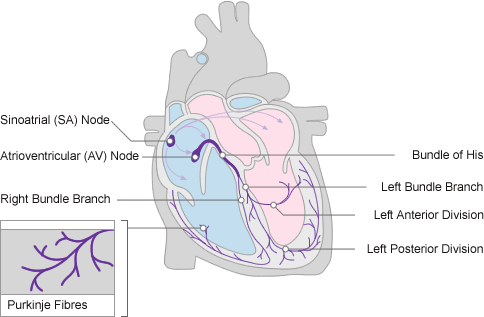
\includegraphics[width=0.8\textwidth]{cardiac_conduction}
  \caption[Pattern of electrical activation in the heart]{Schematic outline of the sequence of electrical activation in the mammalian heart. Image originally downloaded from www.nottingham.ac.uk on 10th December 2012.}
  \label{fig:conduction-pattern}
 \end{figure}
 
 \subsection{Electrophysiological Properties of Cardiomyocytes}
 \label{subsec:electro-prop}
 As previously stated, the main r\^ole of the heart is to serve as a pump to circulate the blood around the body. To do this effectively, it requires coordinated contraction, and this is achieved through the use of coupling the electrical activity of the heart of the mechanical activity (the details of this mechanism will be expanded upon in \S\ref{subsubsec:ecc}).
 
 Physically, cardiomyocytes are typically $10-20\mu$m in diameter, and $50-100\mu$m in length. They are cells bound by a lipid bilayer membrane, separating intracellular space (containing the cytoplasm, nuclei and other organelles) from the extracellular space. The intracellular space has a very different composition to the extracellular space, with the intracellular space containing a high and low concentration of potassium (\K) and sodium (\na) ions respectively; the reverse is true for the extracellular space. These concentration differences are the main reason behind their being an electric potential difference set up across the cell membrane, referred to as the \emph{membrane potential} ($V_m$); this potential is defined as negative when the intracellular space contains a greater negative charge than the extracellular space. At rest, due to the high \K{} and low \na{} in the cell,this potential is negative, though the magnitude varies depending upon the location in the heart; a cardiomyocyte in the ventricles typically has a resting potential ($V$\sub{rest}) of about $-80$mV, while the sinoatrial node has a resting potential of between $-50$ and $-60$mV.
 
 Embedded within the bilayer are various membrane-bound proteins which serve to transport ions across the membrane, allowing the membrane to be selectively permeable to particular ions, and allowing regulation of this permeability as required. These transporters can be classed as either \emph{channels} (allowing ions to move according to their electrochemical gradient), \emph{pumps} (translocating ions in the opposite direction to their electrochemical gradient by the use of energy) or \emph{exchangers} (translocates a number of ions of one type across the membrane in `exchange' for a number of ions of another type). Most of these transporters are ion-specific, though some are not exclusively selective. Most of these channels are also controlled by, amongst other things, the membrane potential itself \citep{Bezanilla2000}. The membrane potential causes a conformational change in the ion channel protein, causing it to `open' or `close'; that is, to allow ions to be conducted through it or not.
 
 These ion channels are discrete molecular entities, and thus the conformational changes that lead to their open/close state are stochastic; the effects of this stochasticity are discussed in greater detail in \S\ref{sec:param-var}. However, each type of ion channel possesses its own range of attributes, such as the time it takes to inactivate, the time it takes to reactivate, its permeability to different types of ions, and its susceptibility to other gating factors. Comprehensive summaries of the properties of ion channels are given in \citet{Carmeliet2002, Roden2002}.
 
 Electrically, the heart can be modelled with great success as an analogue to an electrical circuit \citep{Carmeliet2002}, where the lipid bilayer is represented as a capacitor, and the various ion channels and transporters that span the membrane are represented as resistors, which change their `resistance' depending on their state. By altering the resistance of these channels, ion flow across the membrane is permitted via an ionic current. It is a point of nomenclature that an `inward' current represents the movement of positive ions from the extracellular to the intracellular space, and an `outward' current is the reverse. This definition is based on the movement on electrical charge, and not on the movement of ion flow. This is subtly different to the definition of an inward or outward rectifier current, where an inward rectifier current passes current more easily inward than outward, and vice versa for an outward rectifier current.
 
 \subsubsection{The Action Potential}
 \label{subsubsec:ap}
 The changes in internal/external ion concentrations which result from these currents changes $V_m$. The cyclic, periodic change in membrane potential is referred to as the \emph{action potential} (AP). An example of an action potential, showing the different `phases', is shown in Fig.~\ref{fig:ap-structure}. 
 \begin{figure}
  \centering
  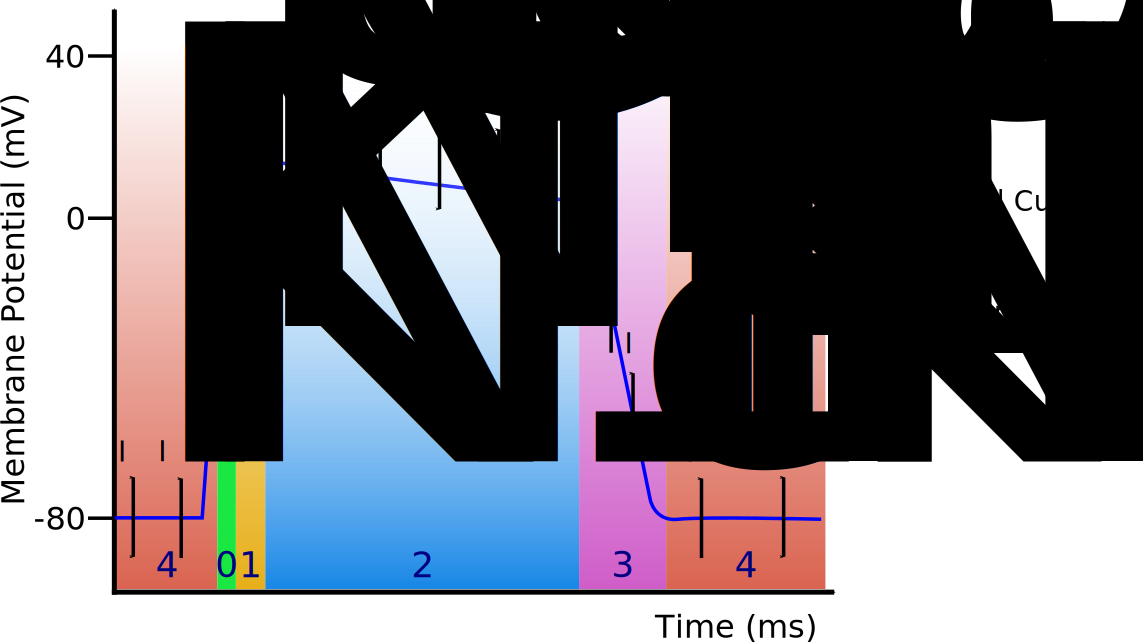
\includegraphics[width=0.8\textwidth]{ap-structure-full}
  \caption[Schematic of a cardiac AP]{Schematic of a ventricular cardiac AP, with the different `phases' of the AP shown, and which key currents are involved in each phase. Upward arrows represent outward currents, inward currents represent inward currents, and double arrows represent exchangers, \idest{} where current moves in both an inward and outward direction.}
  \label{fig:ap-structure}
 \end{figure}
 
 The AP is considered to consist of 5 different phases, outlined below. The important currents in each phase are mentioned, and greater details are given for a number of these current in \S\ref{subsubsec:channel-dynamics}.
 \begin{description}
  \item[Phase 4:] The resting phase. For ventricular and atrial cardiomyocytes, this phase is marked by a relatively constant value for $V_m$. The negative resting potential is largely achieved by the inwardly rectifying potassium current (\ikix{}) remaining open during this phase. For pacemaker cells, \ikix{} is absent, and thus the resting phase is actually a period of slow depolarisation, until $V_m$ reaches the threshold value for phase 0. There is also an inward current due to the \na{}-\ca{} exchanger current (\inaca), which moves 3 \na{} ions into the cell and one \ca{} ion out at the resting potential.
  \item[Phase 0:] Period of rapid depolarisation that marks the start of the AP. It is initiated by $V_m$ reaching a threshold value which causes the \ina{} current to activate, causing a rapid influx of \na{} into the cell. In response to this, the direction of \inaca{} reverses, and this newly outward current brings in \ca{} and removes \na{}.
  \item[Phase 1:] Transient repolarisation. The \na{} channels rapidly deactivate (the process leading to reactivation does not start until the cell repolarises at the end of the AP), and the activation of the transient \K{} outward current (\ito{}, occasionally referred to as $I_{\textnormal{to1}}$) results in a period of rapid, partial repolarisation. There may also be a contribution from a \ca{}-activated \cl (\icacl, or $I_{\textnormal{to2}}$). Depending on the strength of this current, this repolarisation may be to the extent that there is a `notch' in the AP, where the cell transiently repolarises beyond the susbequent plateau phase potential. For example, there is a notch in the AP for ventricular epicardial cells, but no notch for ventricular endocardial cells. The characteristics of this phase are also species-dependent \citep{Carmeliet2006}.
  \item[Phase 2:] Plateau phase. The membrane potential is sustained at a relatively constant level by a balance of calcium (\ca{}) influx via the L-type calcium current (\ica{}), and potassium efflux, through the rectifier \K{} currents (rapid,\ikr{}, and slow, \iks{}). Despite being a rapidly activated current, \ikr{} does not carry large current early during this phase, but only peaks at the end. \ikix{} shows a dramatic fall in conductance during this phase. While most \ina{} is inactivated during phase 1, there is a small contribution from \ina{} when $V_m$ is in the limited range where activation and inactivation both occur. Late during phase 2, due to the increase in \cai{}, the reversal potential for \inaca{} increases to a value greater than $V_m$, and thus \inaca{} returns to being an inward current.
  \item[Phase 3:] Repolarisation. The L-type \ca{} current channels close, while the \iks{} channels remain open, allowing continuing \K{} efflux resulting in a repolarisation of the cell to the original resting potential. \ikix{} opens during this phase, to remain open during phase 4 to maintain a steady resting potential. 
 \end{description}
 It should be noted that the above description of which currents act during which phase is only an outline. While the upstroke of the AP is due mostly to the action of \ina{} and the associated rapid influx of \na{} ions into the cell, causing the rapid depolarisation, the remaining phases of the AP are more complex, and the failure or part failure of any individual component of the cell mechanism does not necessarily lead to the failure of the whole system. This pseudo-redundancy was first termed \emph{repolarisation reserve} in \citet{Roden1998}, and was demonstrated experimentally in \citet{Varro2000}. It is essentially the concept that a loss in repolarisation function caused by a reduction or loss of function in one repolarising current can be recovered by increased action of an alternative repolarising current. Such a loss of function can have many possible causes, \eg{} loss-of-function mutations in the genotype \citep{Rosati2004}. Most often, the term repolarisation reserve is applied to \K{} channels, and specifically for the interaction between \ikr{} and \iks{} \citep{Xiao2008}. Several currents are noted for their r\^ole in maintaining the repolarisation reserve of the cell, some of which have already been mentioned: \ikr{}, \iks{}, \ikix{}, \ito{}, \ica{}, \ina{} \citep{Varro2011}. The repolarisation reserve is not constant, but rather is dynamic with pacing rate, and variable between species and tissues within the heart \citep{Carmeliet2006}.
 
 It is not just the repolarisation reserve that is dynamic, but the entire action potential itself---most notably, there can be significant variations in the AP morphology between different regions of the heart (caused in turn by different ion channel concentrations) \citep{Giles1988}. Beyond this so-called `developmental regulation', it is also possible for the myocyte to adapt to environmental changes, and to ensure the phenotype of the heart is appropriate for the demands placed upon it (`homeostatic regulation') \citep{Rosati2004}.
 
 Even within a particular region of the heart, the AP duration (APD) varies according to the pacing rate. The manner in which the APD varies with pacing rate is often described using a restitution curve, which shows the relation between APD and the \emph{diastolic interval}, which is itself defined according to the quiescent phase of the cell; the sum of APD and DI equals the \emph{cycle length} (CL), \idest{} $\textnormal{APD}+\textnormal{DI}=\textnormal{CL}$. The graphical representation and interpretation of the APD in this manner, with a view to a predicting APD changes after rate changes, was first suggested by \citet{Nolasco1968}.
 
 The APD restitution curve describes the duration of the $(i+1)$-th APD as a function $f$ of the time since the preceding AP, \idest{} the $i$-th DI. This is typically a monotonically increasing function, and can be expressed as $\textnormal{APD}_{i+1} = f(\textnormal{DI}_i)$. If we linearise this around the fixed point $\textnormal{APD}^\ast$, and describe APD as small perturbations round this point ($\textnormal{APD}_i = \textnormal{APD}^\ast+\delta\textnormal{APD}_i$), we can obtain the following (also making use of the Taylor expansion of $f(\textnormal{DI}_i)$ and assuming $\mathscr{O}(\delta\textnormal{DI}^2)$ is small):
 \begin{IEEEeqnarray}{rCl}
  \textnormal{APD}^\ast + \delta\textnormal{APD}_{i+1} & = & f(\textnormal{DI}_i) \\
  & = & f(\textnormal{DI}^\ast) + f'(\textnormal{DI}^\ast)\delta\textnormal{DI}+\mathscr{O}(\delta\textnormal{DI}^2) \\
  & \approx & f(\textnormal{DI}^\ast) + f'(\textnormal{DI}^\ast)\delta\textnormal{DI}
 \end{IEEEeqnarray}
 By recalling that $\textnormal{CL} = \textnormal{APD}+\textnormal{DI}$ and $\textnormal{APD}^\ast = f(\textnormal{DI}^\ast)$, this be further simplified:
 \begin{IEEEeqnarray}{rCl}
  \delta\textnormal{APD}_{i+1} = -f'(\textnormal{DI}^\ast)\delta\textnormal{APD}_i
 \end{IEEEeqnarray}
 Based on this, it can be seen that a bifurcation exists (which manifests as alternans) whenever $|f'(\textnormal{DI})|>1$, due to the amplifying effects of deviations from the fixed point $\textnormal{APD}^\ast$. This is represented graphically in Fig.~\ref{fig:alternans-restitutionCurve}. The gradient of the restitution curve is still of key experimental import, as a steep curve is taken to imply an increased possibility of wave breakup and subsequent fibrillation from tachycardia \citep{Riccio1999}; mechanisms that lead to arrhythmogenesis shall be examined in greater detail in \S\ref{subsec:arrhythmogenesis}.
 
 However, it should be noted that this approach is limited, as it presents the oversimplification that the APD is dependent purely on the preceding DI. Thus, while the resitution curve can be a useful indicator of a tissue's susceptibility to fibrillation and other disorders, it is by no means the only such indicator \citep{Riccio1999}. Furthermore, it makes no account of the \cai{} dynamics---this is discussed further in \S\ref{subsec:arrhythmogenesis}.
 % Monotonic function is one such that, if x<y, f(x) is also < f(y)
 \begin{SCfigure}
  \centering
  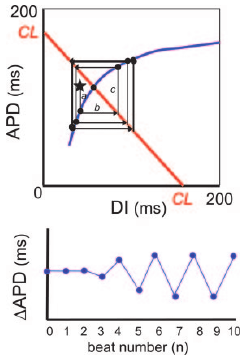
\includegraphics[width=0.5\textwidth]{alternans-restitutionCurve}
  \caption[Example of a restitution curve with alternans predicted]{Example of a restitution curve with alternans predicted. The blue line represents the restitution curve; pacing at a constant CL can be represented by the red straight line. A small perturbation (represented by the star) from the equilibrium point (represented by the circle) can lead to growing perturbations, that eventually settle to alternans. This instability is due to the equilibrium point existing where the gradient is greater than 1. Figure originally from \citet{Weiss2006}.}
  \label{fig:alternans-restitutionCurve}
 \end{SCfigure}
 
 \subsubsection{Ion Channel Dynamics}
 \label{subsubsec:channel-dynamics}
 It should be borne in mind that knowledge of ion channel dynamics is not appropriate solely for cell simulations, but is important for the implications of how such changes cascade through the different spatial and temporal scales. Thus, knowledge of how ion channel dynamics affects cellular AP dynamics leads to knowledge of tissue dynamics implications, and so on \citep{Spach1988}. The emphasis on what follows is on the ion channel dynamics of rabbits---while there are many similarities in these channels between mammalian species, it is important to remember that species differences can be significant \citep{Bassani1994}. For example, \ito{} plays an important r\^ole in repolarisation in rodents, and thus strongly influences APD, while playing a relatively minor r\^ole in repolarisation in larger mammels \citep{Rosati2004}.
 
 \ikr{}, as the name implies, is the more rapidly activating of the two rectifier \K{} currents ($\tau\sim40$ms at $+30$mV), and rapidly activates once $V_m$ increases above $-30$mV. However, the channel inactivates even more rapidly in a process that precedes voltage-dependent inactivation \citep{Varro2011, Spector1996, Carmeliet2006}. Due to this, \ikr{} channels are largely closed during the plateau phase of the AP, only reopening when $V_m$ returns to about 0mV. The transient nature of the current is due to its rapid recovery from inactivation, and subsequent slow deactivation. At slow rates, the contribution of \ikr{} diminishes further, resulting in a positive feedback look regarding prolongation of the AP duration (APD) (the same is observed for \ikix{}) \citep{Virag2009}. This same vulnerability of the repolarisation is evident when depolarising factors (\eg{} \ina{}, \ica{}) are augmented or repolarising factors (\eg{} \iks{}, \ikix{}) diminished.
 
 If the function of \ikr{} is impaired substantially in some way, APD is measured to be significantly prolonged, both by direct measurement of the membrane potential, and QT interval measurements in electrocardiograms (ECGs)  (the QT interval serves as a marker for the time taken for ventricular depolarisation and repolarisation in a clinical setting \citep{Yan1998}), suggesting especial importance in cellular repolarisation \citep{Varro2000, Lengyel2001, Jost2005}. When \ikr{} is only impaired in a minor way, APD may not necessarily increase due to the action of the repolarisation reserve. \ikr{} passes via a channel encoded by the human ether-\'a-go-go related gene (HERG), and is known for being its susceptibility to the effects of drug block, making it of key pharmocological importance \citep{Vandenberg2001, Haverkamp2000}. It can also be noted that, in spite of what may be predicted by the Nernst potential for \ikr{} (see \S\ref{subsubsec:nernst}), increased extracellular \K{} is known to enhance \ikr{} \citep{Sanguinetti1992, Yang1997}.
 
 \iks{} takes longer to activate than its partner (500-1000ms at plateau phase), and deactivates rapidly at negative $V_m$ \citep{Jost2005, Varro2011}. It carries a slowly rising current over the duration of the plateau phase. At rapid pacing rates, the current carried by the \iks{} channel increases---this is thought to be due to the kinetics of the channel, with an `inactivated' state being intermediate between the open and closed state. At rapid pacing rates, there is less time to transition fully to the closed state, and thus there is a greater proportion of \iks{} channels available for immediate opening \citep{Silva2005}. \iks{} is also modelled as having a sensitivity to \cai{}, replicating the results of potassium currents' sensitivity to \cai{} \citep{Meech1975}.
 
 Drug block of \iks{} causes AP prolongation, but not to the same extent as \ikr{}; while direct measurements show a slight increase in APD, there is very little or no change in QT intervals ECG measurements \citep{Varro2000, Lengyel2001, Jost2005}. This implies that its amplitude, compared to that of \ikr{}, during a typical AP is small---this has been confirmed experimentally under normal conditions \citep{Varro2011}. Combined with its slow activation, there is thus relatively little \iks{} active during the AP \citep{Jost2005}. However, its long activation time also means the effect of \iks{} block is more pronounced when APD is prolonged, due to (i) the net outward current at long pacing rates is smaller, so the fractional effect of \iks{} is greater, and (ii) more channels are activated during a long AP \citep{Carmeliet2006}. Due to this action, and the response of \iks{} to sympathetic stimulation, the current provides a negative feedback for APD prolongation, acting to curtail the increased action of \ica{} that occurs at longer pacing rates. Thus, while under `normal' circumstances \iks{} has limited effect on the repolarisation reserve of the cell, it acts as an effective buffer when APD is longer than normal.
 
 The transmural differences in the expression of \iks{} is a large reason behind the transmural variation of APD, and also explains why \ikr{} block can have a greater or lesser effect, depending on the abundance of the compensatory effect of \iks; the scarcity of \iks{} can be noted in Purkinje fibres and M-cells, while it is abundant in subepicardial and subendocardial cells \citep{Vandenberg2001, Carmeliet2006}. The density of \iks{} channels has also been shown to increase in response to sustained \ikr{} block, demonstrating its importance to the repolarisation reserve \citep{Xiao2008}.
 
 \ikix{} is a strongly inwardly rectifying \K{} current, which means that when $V_m$ is greater than $-30$mV, the channel is inactivated. Thus it plays a negligible r\^ole during the plateau phase of the AP, but has a self-reinforcing role in the repolarisation of the cell once $V_m$ decreases to the extent that \ikix{} can be activated. It should be noted that this is not a voltage-dependent activation, but is based on an unblocking of the channel: when $V_m > -30$mV, the channel is blocked by \mg{} and polyamines which enter the channel from the intracellular side in a voltage-dependent manner. As the current is fully open at $V$\sub{rest}, it resists depolarisation caused by either increased pacemaker activity, or \ca{} overload-related delayed afterdepolarisations (DADs). Consequently, \ikix{} may be considered to play an unusual r\^ole in the repolarisation reserve, and impairment of its function could lead to proarrhythmic effects by making the cell more susceptible to extrasystoles.
 
 \ito{} is actually composed of two separate currents, a rapidly recovering component (\itof{}) and a slowly recovering component (\itos{}). As a combined unit, it both activates and inactivates rapidly for $V_m > -20$mV, and is of greatest importance during the phase 1 repolarisation. As such, it is believed to have little influence directly on the end repolarisation of the cell, but due to its early role, and its consequent effect on the plateau potential, it is believed to have influence on subsequent currents, which lead to great indirect influence. \ito{} is also known for its transmural variation, being greater in epicardial than endocardial tissue.
 
 \inak{} is caused due to the \na{}-\K{} pump, which is an electrogenic exchanger, moving 3 \na{} ions out of the cell in exchange for 2 \K{} ions. It thus works to maintain the concentration gradients and the resting membrane potential, and provides an outward current in support of the repolarisation reserve. It is, however, sensitive to intracellular \na{} concentration (\nai), and consequently to the rate of stimulation.
 
 The influence of \ica{} on the repolarisation of the cell is complex due to its complicated inactivation. It inactivates due to voltage slowly, and thus the main reason for its inactivation is due to \ca{}-induced inactivation, and is thus in response to local \ca{} concentration, which is dynamically changing during the plateau phase. This inactivation is modulated via a protein called calmodulin, and thus can be modulated further. If the AP is extended during the range of activation/inactivation for \ica{}, some \ica{} channels may reactivate. This resurgence of the inward current can lead to secondary depolarisations or early after-depolarisations (EADs) \citep{Carmeliet2006}. 
 
 It should be noted that \ica{} is a highly localised current---the responsible channels are not distributed uniformly throughout the sarcolemma, but are instead localised to close proximity to other channels important in the contractile mechanism of the cell, serving to co-ordinate the release of \ca{} throughout the cell; this is explored in greater depth in \S\ref{subsubsec:ecc}. This localisation is not unique to \ica{}---it has recently been demonstrated that \ina{} is also highly localised \citep{Bhargava2013}.
 
 If \ica{} (or \ina{}) are augmented and have their activity increased, this serves to make the plateau potential more positive. While at first glance this may indicate that AP may lengthen, it is rather the case that this may serve to enhance activation of outward \K{} currents, thus shortening APD.
 
 The \na{}-\ca{} exchange current (\inaca{}, also referred to as \incx{}), like \inak{}, is an electrogenic exchanger, this time exchanging 3 \na{} ions for one \ca{} ion. By this process, it is, with the SERCA pump, largely responsible for restoring the low cytosolic \ca{} concentration during diastole; it is the main means for extruding \ca{} from the cell, responsible for $70-90\%$ of the \ca{} efflux \citep{Eisner2004}. Despite this, the activity of \inaca{} can be inhibited by $80-90\%$ with cardiac function still being maintained \citep{Henderson2004}---another example of effective repolarisation reserve. \inaca{} depends strongly on $V_m$ and \cai{} \citep{Clusin1983}, and thus its magnitude during the AP is difficult to estimate (a problem compounded by the lack a specific inhibitor for the current). It is an outward current at the start of the AP, when $V_m$ and \cai{} are both low, but then changes to an inward current during the late plateau phase. Due to its sensitivity to \cai{}, in times of \ca{}-overload \inaca{} can provide a depolarising current, thus increasing the likelihood of DADs and EADs \citep{Clusin2003}. The density of \ina{} is also known to depend heavily on \cai{}, decreasing when \cai{} is high; the gating of the channel is not affected.
 
 These, and other, currents are susceptible to alteration, and demonstrate varying degrees of importance during physiological and pathological conditions; the arrhythmogenic properties of some of these currents will be discussed further in \S\ref{subsec:arrhythmogenesis}.
 
 \subsubsection{Excitation-Contraction Coupling}
 \label{subsubsec:ecc}
 Arguably, the complex electrical activity of the AP just described exists for the sole purpose of ensuring the heart acts as an effective mechanical pump. As such, the linking of the electrical activity of the heart to its mechanical contraction is vital, as is referred to as \emph{excitation-contraction coupling}. What follows is a brief summary of the mechanism of this link (the reverse side of this mechanism, termed mechanoelectric feedback, shall not be discussed here). More details of the mechanical aspect of the cardiac cycle, and of the attempts to model it and integrate it with electrical models, can be found in \citet{Trayanova2011}. A summary of \ca{}-handling in the cell is provided by \citet{Eisner2000}.
 
 For this discussion, the cell may be decomposed into units called calcium release units (CRUs), also known as dyads \citep{Cleemann1998}. These CRUs are spread roughly evenly throughout the cell to allow for a uniform action throughout---the number of CRUs in the cell has been estimated to be between 10,000 and 100,000 \citep{Cleemann1998,Greenstein2002}. Anatomically, the CRU may be considered to be a section of the cell containing a section of the cell membrane, with some L-type \ca{} channels, and a section of the sarcoplasmic reticulum (SR). The primary r\^ole of the SR is to sequester and release \ca{} when the required stimulus is given. This release is predominately by \emph{ryanodine receptors} (RyR), but at least one other channel (Inositol triphosphate-activated channels, or IP$_3$) is known to play a part, and others are reported \citep{Pozzan1994}. This stimulus is the rise in local concentration of \ca{} precipitated by the opening of the L-type \ca{} current channels, and is termed \emph{calcium-induced calcium release} (CICR) \citep{Fabiato1992}. The result is that a great deal of \ca{} is released into the cytosol of the cell during phase 2 of the AP under `normal' conditions. It can thus be noted that the \ca{} system of the cell is dependent on the AP, which is in turn affected by the \ca{} dynamics (both due to the positive charge associated with \ca{}, and due to \ca{}-sensitive membrane currents, \eg{} \ica{} \citep{Weiss2006}. The release of \ca{} from the SR is modulated by means of a \ca{}-binding protein within the SR called calsequestrin (CSQN)---computational modelling of its effects by \citet{Restrepo2008} demonstrate that this is behind the steep load-release relationship exhibited by SR release.
 
 The reason this is vital for ECC is due to the interaction between \ca{} and the contractile units of the cell, called the sarcomere. When the cytosolic concentration of \ca{} (\cai{}) rises, the free \ca{} binds to a part of the contractile machinisms of the cell, which then removes the inhibition between the two critical contractile parts of the mechanism, allowing contraction to take place. It should be remembered that the \ca{} transients \emph{precede} contraction, and the upstroke velocity of the transient is faster than the rise in force \citep{Lee1988}.
 
 Subsequent to contraction, the \ca{} released from the SR is recovered by the sarco/endoplasmic reticulum \ca{}-ATPase pumps (referred to as SERCA) \citep{Franzini-Armstrong2005} (which is inhibited by a protein called phospholamban, among other factors \citep{Talukder2009, Xu1993, Eisner2000}). Further \ca{} is extruded from the cell by \inaca{} \citep{Laurita2008} (it should be noted that \inaca{} brings in 3 \na{} ions for every \ca{} ion extruded, making it an eletrogenic current). Other mechanisms for removing cytosolic \ca{} are negligible \citep{Bassani1994}. At steady state, the influx from \ica{} and the efflux from \inaca{} are equal. When not in steady state, the value of \cai{}, influenced by SR \ca{} release (and thus SR \ca{} load), operates to return the system to steady state. This process has been referred to as `autoregulation' \citep{Eisner2000}.
 
 The end \cadia{} is heavily dependent on this uptake/extrusion process---if there is an inhibition/upregulation of either process, it can have a significant beat-to-beat effect on \cadia{}. It should be noted that neither the reduction of \cai{}, nor the involved buffering, are not linear processes. \citet{Bers1995} demonstrated a that SERCA demonstrates Michaelis-Menten kinetics in the buffering/sequestration process---this is ideal for the requirements of the system, in that it increases the rate of decay of \cai{} when \cai{} is increased, \idest{} if the \ca{} transient is greater, the cell is able to return \cai{} to a diastolic value within a similar amount of time as for a small transient.
 
 There is a long-known association between alternans in the \ca{}-handling mechanisms of the cell and arrhythmias, on the basis of the feedback between the \ca{} system and the AP itself. However, the precise mechanism, and the causal links involved, are still the topic of much debate, and work is ongoing to establish the means by which alternans and arrhythmias are linked \citep{Alvarez-Lacalle2013, Chen2009, Restrepo2008}. More details as given in \S\ref{subsubsec:alternans}.
 
 % Additional details (not sure if required for thesis):
 % Decreased activation/inactivation of RyR -> alternans (Alvarez-Lacalle2013). Increased stimulation frequency reduces required decrease activation/inactivation. Clamping SR Ca eliminates decreased inactivation alternans
 
 % Steep relation between SR load and SR Ca release (Shiferaw2003) - see Gemmell2010 (transfer thesis) for more details
 
 % Details of Ca SR releease dependence: Laurita2008
 
 \section{Computational Cell Models}
 \label{sec:cell-models}
 It is often not practicable to test hypotheses in full experimental conditions. Under such circumstances, computational/mathematical models have become increasingly important in recent years, as they have developed from their original humble origins \citep{Jalife2013}. The focus of computational models can be broken down to three areas of scale: the cellular, the tissue, and the organ. It should be noted that there is considerable overlap between each of these scales, and it would be a mistake to think of models other than cellular models as entirely being tissue or otherwise models.
 
 There are three key methods for computational modelling of the heart, each appropriate for different scales and different hypotheses. They are, in order of computational complexity: eikonal modelling, phenomenological modelling and ion channel modelling. Eikonal modelling (which can only be used with any accuracy on length scales greater than that of individual cells) concerns itself with modelling the spread of the action potential wave by modelling the wave propogation directly, without attempting to recreate the AP itself \citep{Keener2009}. Phenomenological modelling attempts to recreate the AP directly using differential equations adapted specifically for the AP \citep{Bueno-Orovio2008}. Finally, ionic models attempt to recreate in a biophysically detailed manner the ion currents involved in the creation of the AP. This is the most computationally intensive of the three approaches, but allows a wide range of hypotheses to be addressed. Each of these modelling approaches bring their own series of benefits and costs, with implications based on the trade-off between computational complexity and biophysical detail. It should be remembered that a biophysically detailed ionic model has, almost be necessity, a large number of parameters to fit to match the data, and fitting these parameters increases not only the complexity, but also the possible sources for error \citep{Relan2011}.Ionic models are the focus of this thesis.
 
 Great advances have been made in accurately modelling individual ion channels, assessing the importance of stochasticity, and probing the interplay between systems and levels in complicated simulations. What follows is a summary of some of the key concepts that are of use in computational models in \S\ref{subsec:model-concepts}, and then a brief background on the evolution and development of computational cell models from their early days in \S\ref{subsec:model-development}. Various difficulties and problems in model construction that need to be borne in mind when using such models are outlined in \S\ref{subsec:model-difficulties}.
 
 When considering computational models, it is worth remembering that, from the outset, a model is \emph{wrong} in some way---it is useful insofar as it can answer a posed question. A good model will be able to address a wide range of questions, and will direct future research. This is not necessarily a bad thing---much can be learned from the failure of models, as well as from the success \citep{Noble2001, Quinn2013}. Indeed, computational models are a natural extension of the usual scientific process: a hypothesis is conceived, a model designed to test the hypothesis, and thus the hypothesis is either validated, and further questions may be asked, or falsified.
 
 \subsection{Key Concepts}
 \label{subsec:model-concepts}
 The model's purpose defines what variables are considered, and how these variables are determined. Some models (\eg{} \citet{Restrepo2008}) define a certain section of the cellular mechanism as of interest, and thus the output is defined accordingly. However, most models are trained according to the membrane potential, and thus that is considered the primary output. In modelling the cell as an electrical circuit with the membrane considered as a capacitor, the instantaneous change in membrane potential is calculated according to
 \begin{equation}
  \frac{\textnormal{d}V_m}{\textnormal{d}t} = -\frac{1}{C_m}(I_{ion}+I_{stim}),
 \end{equation}
 where $C_m$ is the membrane capacitance, $I_{ion}$ is the sum of all ionic currents in and out of the cell, and $I_{stim}$ is the stimulus current, if applied, to initiate an AP. In experiments and simulation, the value of \istim{} can vary, but it is usually at least $1.5$ times the minimum value required to initiate activation (the activation threshold) \citep{Sutton2000, Riccio1999, Ferrero2003}.
 
 It should be noted that the membrane potential method can also be calculated according to an 'algebraic method', based on the charge conservation principle and the charge-voltage relation of a capacitor; identical results are produced by both methods \citep{Hund2001, Rudy2006}.
 
 In biophysically detailed models of electrically excitable cells, most ionic currents are modelled according to:
 \begin{equation}
  I_X = g_X(\mathbf{x})(V_m-E_X),
 \end{equation}
 where $I_X$ represents the ionic current being modelled, $g_X(\mathbf{x})$ represents the conductance of the channel and $E_X$ represents the Nernst potential, also known as the reversal potential of the cell. This is the potential at which there is no net ion flow through the channel, \idest{} there will be no ionic current. The general form of $E_X$ is explained in \S\ref{subsubsec:nernst}. $g_X(\mathbf{x})$ is current-dependent variable, and can be modelled as varying with time, voltage, extra-/intracellular ion concentration, etc..
 
 \subsubsection{Nernst Potential}
 \label{subsubsec:nernst}
 Of key importance in mathematical modelling of electrically active cells is the \emph{Nernst equation}. A full derivation is given in the appendix, but the key result is thus:
 \begin{equation}
  E_X = \frac{RT}{z_XF}\ln\frac{[X]_\textnormal{o}}{[X]_\textnormal{i}}
 \end{equation}
 In the above equation, $R$ represents the gas constant, $z_X$ represents the valence of ion $X$, $F$ represents the Faraday constant, and $[X]_\textnormal{o}$ and $[X]_\textnormal{o}$ represent the extracellular and intracellular concentrations of $X$ respectively. The quantity of interest, $E_X$ is the \emph{Nernst potential} or \emph{reversal potential}, and represents the value of $V_m$ required to maintain the intra-/extracellular concentration ratio constant, \idest{} to make the net ionic flux across the cell membrane zero.
 
 When a channel is entirely selective, the reversal potential (which can now be thought of as the potential at which there will be no net flux of ions) is given by the Nernst equation for the specific ion. However, some ion channels are permeable to more than one type of ion, in which case their reversal potential for channel $\alpha$ is given by the \emph{Goldman-Hodgkin-Katz equation}:
 \begin{equation}
  E_\alpha = \frac{RT}{F}\ln\frac{\Sigma_i^N P_{A_i^+}[A_i^+]_\textnormal{o} + \Sigma_j^M P_{B_j^-}[B_j^-]_\textnormal{i}}{\Sigma_i^N P_{A_i^+}[A_i^+]_\textnormal{i} + \Sigma_j^M P_{B_j^-}[B_j^-]_\textnormal{o}}
 \end{equation}
 The above equation describes the situation for $N$ different monovalent positive ionic species and $M$ monovalent negative ionic species; different valencies complicate matters further.In it, $E_\alpha$ represents the reversal potential for the channel, \idest{} the potential at which, with the given ion concentrations, no net electric flow will occur. The permeability of the membrane is given by $P_X$; as with the concentrations, the terms have been split into positive ($A_i^+$) and negative ($B_i^-$) ionic terms.
 
 \subsubsection{Hodgkin-Huxley Current}
 As previously stated, the seminal work presented in \citet{Hodgkin1952} modelled currents as being composed of one of more activation/inactivation gates. It should be noted that the original paper was at pains to emphasise that this was not intended as a description of the actual, physical channel, but was to be used as is: as a mathematical equation that provides a fidelity to the experimental data. It is of note, however, that it is the case that the structure of the \K{} channel does consist of four identical subunits, which does correspond with the four gating variables required in the Hodgkin-Huxley formulation of the current.
 
 Within the Hodgkin-Huxley framework, the current conductance can be modelled according to
 \begin{equation}
  g_X = \overline{g}_Xm^a h^b,
 \end{equation}
 where $\overline{g}_X$ represents the maximum conductance through the channel, $a$ and $b$ are constants, $m$ represents the activation gate and $h$ the inactivation gate. In \citet{Hodgkin1952}, a physical basis was given to $m$ and $h$ by describing them as proportions of `activating molecules' and `inactivating molecules', respectively---the conductance through the channel is thus proportional to the proportion of these molecules that are within and outwith the cell. The change in these variables are described according to
 \begin{equation}
  \frac{\textnormal{d}m}{\textnormal{d}t} = \alpha_m(1-m)-\beta_m,
 \end{equation}
 where $\alpha_m$ and $\beta_m$ are functions of $V_m$. It can be noted that this is often expressed as
 \begin{equation}
  \frac{\textnormal{d}m}{\textnormal{d}t} = \frac{m_\infty-m}{\tau_m}
 \end{equation}
 where $m_\infty=\frac{\alpha_m}{\alpha_m+\beta_m}$ and $\tau_m=\frac{1}{\alpha_m+\beta_m}$, and are the steady state value of $m$ and the time constant, respectively.
 
 \subsubsection{Markov Models}
 \label{subsubsec:markov}
 The Hodgkin-Huxley formulation is computationally efficient, but does not represent a physical reality of the channel state. As such, it is poorly suited to model state specific processes, such as mutation effects or stochasticity \citep{Adeniran2011}. It also relies on the independence of the activation and inactivation processes---the formulation assumes these depend only on $V_m$. However, this assumption is not always valid: inactivation of \ina{} has a greater probability of occurring when the channel is open \citep{Bezanilla1977, Armstrong1977}.
 
 To address these limitations, \emph{Markov modelling} can be used (it should be noted that in the formalism presented here, it is not suited to modelling stochastic processes, but can be adapted to do so). Markov modelling works by assuming that the channel can exist in any one of $n$ discrete states, \idest{} it attempts to directly model the ion channel state. These states can be open, closed or inactivated, and there can be multiple types of each state. The simplest form is a two state system, such as
 \begin{center}
  \ce{C <=>[\ce{$k_\textnormal{on}$}][\ce{$k_\textnormal{off}$}] O},
 \end{center}
 where $k_\textnormal{on}$ and $k_\textnormal{off}$ represent the transition rates between these two states---in cardiac modelling, these transition rates typically depend only on the membrane potential. The key requirement for a Markov model is the \emph{Markov property}, which states that the transition to the next state depends only on the current state, and there is no cumulative history of the system that influences its future. Thus, if $x_i(t)$ represents the proportion of channels in state $i$ at time $t$, and $k_{ij}$ represents the transition rate from state $i$ to state $j$, the transition rates for a system containing $m$ different states may be modelled according to
 \begin{equation}
  \frac{\textnormal{d}x_i}{\textnormal{d}t} = \sum_{j=1}^m (k_{ji}x_j - k_{ij}x_i).
 \end{equation}
 The conductance of the channels for a particular current is thus calculated by multiplying the maximum conductance by the proportion of the channels that currently exist in an open state. It should be noted that, when the transitions between states are independent, the Markov formulation devolves to the Hodgkin-Huxley formulation---for further details, see \citet{Rudy2006}.
 
 \subsection{Development}
 \label{subsec:model-development}
 What follows is a summary of the progression and development of computational cardiac models. For further details of the models themselves, the reader is referred to the original papers, and for more in depth summaries of the development, the reader is referred to the reviews given in \citet{Noble2001, Noble2012, Noble2011, Puglisi2004, Rudy2006, Niederer2009}.
 
 The precursor to all computational models of cardiac cells was the model developed in \citet{Hodgkin1952}. This model described the electrical acitivity of a giant squid axon. It described the ionic currents required to explain the change in membrane potential, using a model for each current of a series of activation and inactivation gating variables (details given in \S\ref{subsec:model-concepts}). This model was able to sufficiently model the AP of the neuron using only three ionic currents: a \K{} current, a \na{} current, and a `leak' current of other ions. It was further developed by \citet{Fitzhugh1960}, which even then recognised that, while the `truth' of the model was not universally accepted, the model nonetheless was successful in reproducing experimental results. However, FitzHugh was able to demonstrate that, with the correct adaptations of the model equations, the output could be altered to reproduce the longer APs of cardiac cells.
 
 The Hodgkin-Huxley model was hugely successful, and paved the way for the extension of the computational modelling approach to cardiac cells. Preliminary work was shown in \citet{Hutter1960, Noble1960}, which presented an adaptation of the Hodgkin-Huxley model for the AP of cardiac pacemaker cells. The same 3 currents were used, with adaptations in \ik{} to reproduce the longer AP of cardiac cells. The model was subsequently refined and expanded to reproduce the AP of Purkinje fibre cells \citep{Noble1962}, taking into account experimental data demonstrating the existence of at least two \K{} currents (labelled $I$\sub{K}~and $I$\sub{K1}) with the resulting change in \K{} permeabilities of the cell membrane \citep{Hutter1960, Carmeliet1961, Hall1963}.
 
 This model was followed by a model designed to reproduce the AP of a ventricular myocyte \citep{Krause1966}. The Noble and Krause models were both based on the Hodgkin-Huxley model, with the Noble model being used as the seed for future developments in the computational cardiac modelling field. The next major refinement of the model came with that proposed by \citet{McAllister1975}. In response to experimental data, this model greatly expanded the number of ion channels that were being modelled---the previous 4 ODEs of the Noble model were now replaced with 10. This included modelling the componenets of \ik{} separately as \ikr{} and \iks{}, as well as incorporating a \ca{} current based on experimental recordings from patch clamp experiments. This model, despite its success in reproducing experimental data, also contained an impressive flaw, in that it posited the slow conductance changes near the resting potential to an outward current, activated by depolarisation. In fact, the change was due to an inward current activated by hyperpolarisation (the so-called `pacemaker current' (\iF{})). Despite this flaw, the overall model remained sound, and iterations of the current continued through to \citet{DiFrancesco1985}, which was the first model to incorporate a formulation for the \na{}-\K{} exchanger, and made most intracellular ion concentrations dynamics. It also managed to model SR \ca{} release, and demonstrated the stoichiometry of the \na{}-\ca{} exchanger had to be 3:1, not 2:1 as had previously been supposed---consequently, the resulting current from this exchange (\inaca{}) was incorporated into future models.
 
 While this progress was still being made in the modelling of Purkinje fibre APs, a new focus was found in modelling the AP of ventricular myocytes. While this had already been achieved to some extent in \citet{Krause1966}, the first widely used ventricular model was that proposed in the work of \citet{Beeler1977}. This model was also the first to make more explicit mention of the internal calcium dynamics of the cell, by simulating the \ca{} release from the sarcoplasmic reticulum. Of particular note in the further development of the field is the so-called Luo-Rudy model, first published in \citet{Luo1991}. This model was originally designed to study arrhythmias in guinea pig ventricular cells, but has been subsequently developed for a wide variety of different tasks, and key components have been adapted into other models for other species \citep{Shaw1997a, Shaw1997b, Wagner1999, Viswanathan1999, Garfinkel2000, Shannon2004, Mahajan2008}. Specifically, the model was further adapted in two papers \citep{Luo1994, Luo1994a} to include dynamic intracellular ion concentrations, and \ica{} was reformulated. Significantly, \ik{} was separated into the two constituent currents of \ikr{} and \iks{} in \citet{Zeng1995}, based on experimental evidence for this separation \citep{Sanguinetti1990}. The Luo-Rudy model was also adapted to be able to model isch\ae{}mia by the incorporation of \ikatp{} \citep{Shaw1997} (further details of the modelling of isch\ae{}mia can be found in \S\ref{subsec:ischaemia}). A further significant advance came with \citet{Clancy1999}, which for the first time incorporated Markov modelling into a cell model (Markov modelling is described in greater detail in \S\ref{subsubsec:markov}).
 
 \citet{Stern1992} noted a short-coming of the Luo-Rudy model by its inability to reproduce the graded relationship between \ica{} and the SR \ca{} release---this was due to what was termed the `common pool' model for \ca{}. This can be overcome by introducing a compartmentalised system to model \ca{} dynamics. This allowed for modelling of not only graded \ca{} release (local \ica{} influx causes local SR \ca{} release, which spreads across the cell in a \ca{} wave), but also predicted the phenomenon of \ca{} sparks, which were observed experimentally in \citet{Cleemann1998}. The model was subsequently revised and expanded by \citet{Shiferaw2003} to include SR load-release dependence, although on a purely phenomenological basis. This model has been used as the basis for more elaborate models, incorporating greater biophysical details, including 3D cellular architecture \citep{Restrepo2008, Chen2009}.
 
 It should be noted that almost all currents in the models described above still use the some basic model form as that given in \citet{Hodgkin1952}---details and nuances have been added to some equations, and other equations have been formulated using entirely different methods (\eg{} Markov modelling), but the underlying modelling philosophy has remained rather steady, and been found sufficient to the present day.
 
 It is through this evolution of models from relatively humble beginnings that we have reached the point where we are today---computational models of cardiac systems can be used to model anything from the subcellular to the full organ level, with specialisations depending on species, location and situation. In this thesis, focus is mainly devoted to the models presented in \citet{Shannon2004} and \citet{Mahajan2008}. These are both models for rabbit ventricular myocytes, with the latter model being itself based on the former---they are both in turn based in large part on the Luo-Rudy model. However, it should not be thought that it is a direct step from the Luo-Rudy model to the Shannon model to the Mahajan model---there are numerous intervening steps \citep{Zeng1995, Puglisi2001, Bassani2004}.
 
 Further developments in modelling are constantly being made. Work is also now being increasingly focused on tissue and organ simulations, and the pathologies that one encounters under such situations \citep{PittFrancis2009, Arevalo2007}. Such higher order simulations are computationally far more expensive, and some work has been conducted to investigate the specific effect of tissue level effects \citep{Viswanathan2000}. Molecular simulations are being conducted, but due to their computational intensity, they are limited to ion channel investigations \citep{Nekouzadeh2011}. Work is also ongoing on using bioenergetic considerations to model the system \citep{Niederer2013}. On a purely practical level, work is also increasingly being performed to standardise the computational tools used for simulation, to support reuse of code and replicability of results \citep{PittFrancis2009, Mirams2013}.
 
 \subsection{Difficulties in Model Construction}
 \label{subsec:model-difficulties}
 The first difficulty in model construction is perhaps the most obvious: the data used to construct a model are finite---sometimes surprisingly so, especially if the model is designed to reproduce healthy human hearts. But even if the possible problems of limited sample size are ignored (it is beyond the scope of this thesis to discuss the different possible methods of using data for validation and verification), there are other problems \citep{Marder2011}. One of the foremost problems faced in cardiac modelling is that of scale: the processes involved in the full functioning of the heart can vary across several orders of magnitude ($10^9$ spatially and $10^15$ temporally). It is thus currently impossible to model every single aspect of the heart, and it is essential to use approximations \citep{Abramson2010}.
 
 As shall be expanded upon further in \S\ref{sec:param-var}, variation is a constant in dealing with experimental data, but methods of dealing with this variation are still being developed. Until recently, a model would be designed to reproduce the `data', without reproducing the variation. The choice of what `data' to fit was therefore important, and yet fraught with difficulties. For example, should one fit to the maximum measured value on the basis that voltage-clamp experiments tend to make the currents appear smaller and slower than they are, or should one fit to the mean value in order to use a greater range of data? Both approaches have problems, not least that a model with mean parameters can fail to have properties exhibited by all of the test subjects \citep{Golowasch2002, Marder2011}. Not only does each choice have inherent problems, but the associated variation, expressed often in experimental work as a standard deviation, is often ignored in model construction \citep{Carusi2012}.
 
 A further problem comes with unknown parameters---even in well-studied systems, there are parameters that, for whatever reason, are not well-defined. There are two possible options to deal with this: (1) adopt a parameter derived from a similar system, \eg{} the peak conductance used in a model for a different species, or (2) adjust the parameter on the basis of producing the expected output (so-called \emph{phenomenological fitting}). This problem is especially prevalent for fitting parameters that describe peak/maximum conductance of ion channels; in voltage clamp experiments, it is often the most poorly defined parameter, due to both the possible detrimental effects of the initial cell isolation procedure on ion channels \citep{Yue1996}, and due to the drug block used to try and isolate particular ion channels for measurement being either incomplete or non-specific.
 
 Further difficulties can arise when fitting data due to the experimentally verified repolarisation reserve. While this is a genuine physical phenomenon, when fitting parameters for a computational model, it is possible that, due to the relations between currents and ion concentrations, the model may present with a wide range of possible values that fit the experimental data, with the computational repolarisation reserve being very different to the physiological repolarisation reserve.
 
 \section{Variation}
 \label{sec:param-var}
 Stochasticity has been mentioned in passing already in this dissertation. Stochasticity, and more generally variation, is now being recognised as being of key importance in many biological questions. Variation exists at all ranges, and at all scales. It is at this point that is is useful to draw a distinction between \emph{intrinsic} and \emph{extrinsic} noise/variability. Simply put, intrinsic variability is considered to be due to variation within the system being considered (\eg{} stochastic opening/closing events of ion channels in a cardiac cell), while extrinsic variability is due to changes outwith the system (\eg{} environmental factors). It should be noted that there is the capacity for overlap and thus confusion within this system. For example, environmental factors (extrinsic) can influence the expression of certain genes, but this expression is due to mRNA levels, which are subject to intrinsic variability; as such, extrinsic variability can link to intrinsic variability and \emph{vice versa}, and the dividing line can be blurred. However, the definition given is sufficient for the purposes of this thesis.
 
 % Variability (noun):	The fact or quality of being variable in some respect; tendency towards, capacity for, variation or change
 % Variation (noun):	The fact of varying in condition, character or degree, or other quality; the fact of undergoing modification or alteration, especially within certain limits
 
 %  Use which (surrounded by commas) if a group of words adds information. Use that if it limits the set of things you're talking about. Here are two more examples just to make that clear:
 % Classes that are held on Wednesdays are in building 206.
 % Leap years, which have 366 days, contain an extra day in February.
 % In the first sentence, the words "that are held on Wednesdays" are limiting the type of classes that we're talking about. (We're not talking about all the classes, only the ones held on Wednesdays.) We thus use that. In the second sentence, the words "which have 366 days" are adding information. We thus use which surrounded by commas.
 
 In \S\ref{subsec:experimental-var}, the various possible sources and problems of variation in biological settings are discussed, and in \S\ref{subsec:comp-var}, the various methods used so far to address this variation in computational models are outlined.
 
 \subsection{Experimental \& Physiological Variation}
 \label{subsec:experimental-var}
 As stated, variation exists at all scales, both temporally and spatially: from individual ion channels, to the level of the cell, to tissue, to organ, and to organism. At the scale of ion channels, variation has been noted in the mRNA concentrations that are translated to functional ion channels \citep{Gaborit2007}. While it has been noted that mRNA levels do not translate directly to ion channel concentrations for numerous reasons \citep{Edelman2001, Nattel2010}, a link has still been demonstrated between mRNA levels and observable effects on the AP \citep{Walmsley2013}. There is also a substantial body of evidence for notable variation in cellular processes---in neuronal studies, maximal conductance of ion channels has been shown to vary substantially \citep{Marder2011, Goaillard2009, Schulz2006}, both in theoretical and experimental studies.
 
 As has previously been commented upon, there are notable differences in cellular APs depending the the spatial location on the cell---this is evident from variation between ventricular and atrial (and other) cardiac cells \citep{Carmeliet2002}, to transmural variation \citep{Antzelevitch1991}. Furthermore, temporal variation is also a common phenomenon \citep{Walmsley2010}. At the organ level, numerous factors have been cited as having notable effects on the AP \citep{Taylor1997}. At the organismal level, different individuals react differently to different therapies \citep{Kannankeril2010}. After considering all these changes, there are still notable differences that can be attributed to gender, age, and experimental method \citep{Yang2012, Kurokawa2012}.
 
 A complete and comprehensive discussion of experimental variation is beyond the scope of this dissertation. However, mention shall be made for the experimentally observed variation that is of note for the models and experiments contained within this thesis. The complete gamut of experimental values is almost impossible to find---rather, some measure of the experimental range can be ascertained from the literature by the error values given, which represent the standard deviation of the results from the presented mean value.
 
 \subsubsection{Action Potential Variation}
 \label{subsubsec:ap-variation}
 Collaborators from the University of Szeged have been able to obtain AP traces for ventricular tissue at pacing rates of 600ms and 1,000ms. These preparations are internally consistent---the trace for each preparation comes from a single sample (although the electrode recording the potential occasionally lost contact, and thus had to be reapplied, thus leading to the recording not necessarily coming for the same individual myocyte). These valuable data allow assessment of the intra-preparation variation in AP, and inter-preparation variation. Using data for APD\sub{90}~(arguably the most common AP metric), these data suggest an intra-preparation variability of $\sim3.5\%$, and an inter-preparation variability of $\sim10\%$.
 
 However, these data come from a single laboratory---a full literature review provides a much greater range of values. From these results, it is possible to generate a range of APD\sub{90} values that can be regarded as physiologically realistic. While many of these values come from tissue preparations, preliminary experiments with the Mahajan model suggest that there is little difference between cellular and tissue results for APD\sub{90}. The results of such a literature search gives the physiological range for APD\sub{90} to be $142-185$ms for a CL of 400ms, $160-220$ms for a CL of 600ms, and $167-230$ms for a CL of 1,000ms \citep{Biagetti2006, Szigligeti1996, Yan2001, Jung2011, Goldhaber2005, Wu2011, Wu2008, Wu2008a, Chen2006, Kirchhof2003, Eckardt1998, Zabel1997, Zabel1997a, Kurz1993, McIntosh2000}. Subsequent to these ranges being established and the populations being derived (see Chapter \ref{ch:paramSpace}), further literature was discovered that could expand these ranges further, but not to such an extent that it was felt that the population would change dramatically \citep{Wu2006}.
 
 \subsubsection{Ion Channel Variation}
 \label{subsubsec:ionChannel-variation}
 Many experiments, aware of the added variation associated with differences in gender and age, pick the experimental test subjects to be as homogeneous as possible. Even with that, notable variations can be found. \citet{Fulop2004} used experimental data to determine properties of \ica{}, and found (amongst other details) that the density of peak \ica{} in human ventricular myocytes was $-5.5\pm0.4$pApF\super{-1} ($\pm7.27\%$). Similar values were obtained by \citet{Li1999}, with even greater variation reported for plateau \ica{} (up to $18.2\%$). In the work of \citet{Fink2008}, by fitting to experimental data, \gkix{} was determined to be $0.5871\pm0.0503$pApF\super{-1}mV\super{-1}.
 
 Notable work has also been carried out in \citet{Szentadrassy2005}, which examined the amplitude (and time constants) of several ion channel currents in human and canine tissue to study the inhomogeneities between basal and apical ventricular tissue---a summary of these results is given in Table \ref{table:szentadrassy-results}. It can be seen that the individual results demonstrate significant variation, and variation between apical and basal values is often noteworthy.
 \begin{table}
  \centering
  \begin{tabular}{ccr@{$\pm$}lc}
   Current					& Location	& \multicolumn{2}{c}{Value (pApF\super{-1})}	& Percentage Variation	\\
   \hline
   \hline
   \multirow{2}{*}{\ito{}}			& Apex		& $29.6$&$5.7$					& $\pm19.3\%$		\\
						& Base		& $16.5$&$4.4$					& $\pm26.6\%$		\\
   \hline
   \multirow{2}{*}{$I_\textnormal{Ks,peak}$}	& Apex		& $5.61$&$0.43$					& $\pm7.7\%$		\\
						& Base		& $2.14$&$0.18$					& $\pm8.4\%$		\\
   \multirow{2}{*}{$I_\textnormal{Ks,tail}$}	& Apex		& $1.65$&$0.21$					& $\pm12.7\%$		\\
						& Base		& $0.85$&$0.19$					& $\pm22.4\%$		\\
   \hline
   \multirow{2}{*}{\ica{}}			& Apex		& $-5.85$&$0.76$				& $\pm13.0\%$		\\
						& Base		& $-7.17$&$0.63$				& $\pm8.8\%$		\\
  \end{tabular}
  \caption[Summary of current density results from \citet{Szentadrassy2005}.]{A summary of the results for the current densities of basal and apical ventricular tissue in human and canine myocytes and tissue, obtained from \citet{Szentadrassy2005}.}
  \label{table:szentadrassy-results}
 \end{table}
 
 The effect of gender is addressed in humans in \citet{Verkerk2005}, and in rabbits in \citet{Sims2008}, which also examines the effect of age. The data for humans is not statistically significant, but still shows consistent bias. For example, \ica{} density in female ventricular myocytes is consistently greater than in male at all voltages (\eg{} $129\%$ at 0mV) and for \ito{}, female \ito{} density at 50mV is $84\%$ of the male. The individual measurements in \citet{Sims2008} show up to $9.4\%$ variation in individual measurements, but the gender difference can be far greater---from $22\%$ in prepubertal rabbit ventricular myocytes, to $32\%$ in adult myocytes extracted from the base of the ventricle.
 
 \subsection{Computational Modelling of Variation}
 \label{subsec:comp-var}
 It is a handicap that is only recently being overcome that, in constructing cell models, the focus is on fitting the model output to one particular value, whether this is the mean or some other measure. As such, these models are often poorly equipped to reproduce the variation that is seen in the original experimental data.
 
 When modelling variation, it must be remembered once again that models are only useful up to the point of answering the question posed to them---taking a model further than its original purpose is useful only when this new purpose does not stray irrevocably from the original, and the original models assumptions and approximations remain valid. As such, reproduction of variation using existing computational models is fraught with difficulties when translating the results to the real system. For example,  \citet{Davies2012} showed that by allowing parameters describing peak ion channel conductance to vary, a wide range of possible values could be made to fit experimental AP, with peak conductance varying by factors of 0.1 to 7.43 of the original model's peak conductance value. However, this demonstrates one possible problem in simply fitting parameters: numerically, it may well be entirely accurate, but it may not represent physiological reality (experimental data for conductance variation implies a variation of as much as threefold \citep{Schulz2006}).
 
 As a tangent to this problem of maintaining the link between reality and model, it has been shown that, under particular conditions, a computational model can produce identical AP traces while using two vastly different input parameter sets. However, these models can then differ in other important regards; \citet{Sarkar2010} used two parameter sets for the same model to produce near identical AP traces, but also produced very different data for \cai{}. Obviously, if the model is required only to reproduce the AP, both models are entirely adequate. However, the problem is demonstrated further in \citet{Cherry2007} in a comparison between two different canine ventricular models: while both produce APs of similar morphologies, there are significant underlying differences, and these are reflected in different responses to certain conditions. Similar conclusions have been reached in \citet{Romero2011}, and work has been made in finding some way of curating models according to their differences in response \citep{Terkildsen2008, Cooper2011}.
 
 It is generally felt that a `good' model should be able to reproduce a wide range of data. If a biophysically detailed model can reproduce a wide range of data, it gives us greater confidence that the underlying details of the model can be said to represent reality. By combining a consideration of the model response to different conditions with data regarding the model response to variation, a model's accuracy and efficacy may be assessed, and new experimental directions suggested to either determine which of certain models' hypotheses regarding cell mechanics is accurate, or to elucidate other questions raised.
 
 The interplay between input parameters and output parameters is decidely non-linear, and the effects of changes in one, or many parameters, cannot easily be predicted \citep{Sarkar2012}; this is illustrated in Fig.~\ref{fig:param-var-effect}. The previous modelling paradigm has been to consider the model as occupying a single point in the input/output parameter space---this is represented by the blue point in the figure. However, it is becoming increasingly prevalent to consider variation in both input and output parameter space, represented by the cloud of red points in the figure. However, the mapping between the input and output spaces is non-linear, and there is no guarantee that a point in the middle of the input cloud translates to a point in the middle of the output cloud, or even if the clouds are the same shape (as shown in the figure). This point is worthy of restating: due to the complicated interactions between input components, the effect of a specified change in one input parameter may produce an entirely different effect if other input parameters are altered. Furthermore, the problem increases in complexity as one considers more input parameters and output metrics.
 \begin{figure}
  \centering
  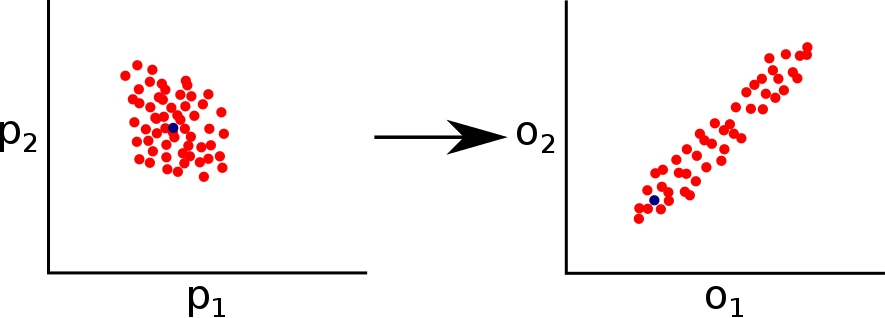
\includegraphics[width=0.8\textwidth]{param-var-effect}
  \caption[Effect of parameter variation on model output.]{Illustration of the effect of possible parameter variation on model output. In this example, two given input parameters ($p_1$ and $p_2$) have a complicated effect on two measured outputs of the model ($o_1$ and $o_2$); one possible example data point is highlighted in blue. Based on a figure from \citet{Sarkar2012}.}
  \label{fig:param-var-effect}
 \end{figure}
 
 There are many different ways to try and elucidate this input/output mapping. One of the more common methods has been \emph{parameter sensitivity analysis}, which varies an individual input parameter at a time to elucidate the effect this parameter has on a given set of output metrics, and expressing this effect in a quantitative manner (\idest{}, $\Delta_\textnormal{output}/\Delta_\textnormal{parameter}$). This work successfully indicates which parameters are most directly responsible for which output metric \citep{Nygren1998, Romero2009, Romero2010, Corrias2011, Romero2011}. This method (and many of the following methods) has obvious extensions to computational predictions for pharmocological ion channel block.
 
 The effects of variation have also been addressed to some degree using stochastic models---\citet{Pueyo2011} has shown that stochastic variation in \iks{}, related to be intrinsic and extrinsic noise, has a measurable effect on APD variation. While such effects are masked by inter-cellular electrotonic interactions in tissue, the effects could become more noted under some pathological conditions, \eg{} intercellular uncoupling due to acidosis. However, both experimental and computational studies of sino-atrial node cells indicate that stochastic fluctuations remain important for observed variation in beat rate \citep{Ponard2007}.
 
 The above methods only provide information for single parameter variation, and biophysically accurate cell models are highly inter-connected, through membrane channel currents' dependence on $V_m$, ion concentrations etc.. As such, with increasing computational power available, more work is being conducted to examine the multi-dimensional parameter space of a model. For a given set $p$ of input parameters (\eg{}, \gnak{}, $\tau$\sub{NaK}, etc.), a range of possible values for each parameter can be defined. There are numerous methods in itself to define this range: it could be based on a percentage range, \eg{}, $\pm15\%$, or based on the range observed for a given parameter in the literature, or by using log-normal distributions of the parameters (the range will equally represent halving and doubling the parameter).
 
 However, as the number of parameters being varied increases, the size of the space increases exponentially. As such, to minimise the computational cost, it is common to survey a sample of the parameter space. There are many ways to extract such a sample, the simplest being a simple random sampling technique. Alternative methods include stratified sampling and Latin hypercube sampling, which attempt to ensure that the parameter space is evenly tested \citep{McKay1979}.
 
 An elegant method to extract the required data from this multi-demonsional sample was demonstrated in \citet{Sobie2009}. For a parameter space surveying the effects of $p$ parameters, a sample of size $n$ parameter sets (where the complete size of the space can be represented by $N$ parameter sets) is selected.Models using these parameter sets are simulated, and the result of these models is recorded according to $m$ output metrics (\eg{}, APD\sub{90}, \casys{}, etc.). Before further analysis, the data are mean-centred and normalised by the standard deviation, \idest{} $x_\textnormal{new} = (x_\textnormal{orig}-\mu_x)/\sigma_x$, where $x_\textnormal{new}$ and $x_\textnormal{orig}$ are the new and original data values, and $\mu_x$ and $\sigma_x$ are the population mean and standard deviation for the data, respectively.
 
 The data are now organised into matrices: the input parameter data are organised into an input $n\times p$ matrix ($\mathbf{X}$), and the output metric data are organised into a $n\times m$ output matrix ($\mathbf{Y}$). Each column thus represents one of the input parameters/output metrics, and each row represents one of the parameter sets simulated, and the resulting output. Multivariable regression analysis is then used to derive the effect matrix $\mathbf{B}$ such that
 \begin{equation}
  \mathbf{XB} = \mathbf{\hat{Y}} \approx \mathbf{Y},
 \end{equation}
 where $\mathbf{\hat{Y}}$ is a close approximation of $\mathbf{Y}$. The result of this analysis is the $p\times m$ matrix of regression coefficients, and has been utilised as each row representing the effect of a given input parameter on the numerous output metrics, and each column representing the effect of various input parameters on a particular output metric. This has been shown to be successful in predicting the output of a new parameter set \citep{Sobie2009}, implying the underlying assumption that the relations remain linear is relatively well-founded while ion concentrations are not varied too much \citep{Sobie2009, Sarkar2010}. The method has also been used to replicate the results of the original parameter sensitivity analysis, \idest{} to demonstrate the effect of a series of input parameters on a given output metric. This method has been used to investigate the effect of such variability on the repolarisation reserve \citep{Sarkar2011}, and also to investigate the possible range of variability in a given set of parameters given the experimentally observed variation in certain output metrics by reversing the regression analysis (\idest{} calculating $\mathbf{B}$ such that $\mathbf{X} \approx \mathbf{\hat{X}} = \mathbf{YB^{-1}}$) \citep{Sarkar2010}.
 
 This method is an elegant method of investigating the effect of multiple parameter variation on multiple model outputs. However, it should be noted that this method still, to some degree, reduces the multi-dimensional parameter variation to a single-dimensional result. The interactions are still tested, and are thus present in an intrinsic sense in the resulting matrix $\mathbf{B}$. Extracting these interactions in an explicit manner is not so simple, and thus the results of the multi-dimensional parameter variation are, in effect, reduced to the result of a single-dimensional parameter variation. It should also be noted that, due to the non-linear effect ion concentrations have on ion-voltage relations, the accuracy of this method may be reduced when concentrations are also allowed to vary. The effect of pacing rate has also not been addressed.
 
 An alternative method is to take advantage of so-called genetic algorithms to tune models to given experimental data. This has been used to provide single parameter sets, and adapt models to new data \citep{Kherlopian2011}. It has also been successfully adapted to find multiple parameter sets that reproduce experimental data, where the parameter sets are not considered part of a continuum of models, with minor variations accounting for the different sets \citep{Achard2006, Syed2005}. While that work reproduced a single set of experimental data, it is not unreasonable to expect this method to be easily adapted to reproduce a range of experimentally observed values.
 
 The effects of multiple parameter variation can also be addressed via a comprehensive parameter sweep (this approach has also been referred to as a database method). The guiding principle of such a method is to comprehensively examine a given parameter space---for example, if the effect of variation in $p$ different parameters is being investigated, the model is simulated for every single possible combination of these parameters. If there are $q$ different possible values for each parameter, this leads to $p^q$ different simulations that would be run, unless measures are taken to limit this by some means (such as by taking advantage of experimentally demonstrated correlations between parameters \citep{Schulz2006}). While this method can be computationally expensive, such a parameter search is also often embarrassingly parallel, and thus can be performed rapidly in real-time using such facilities as the Nimrod computing system \citep{Abramson2000, Abramson1997, Abramson2009, Abramson2010}.
 
 The parameter sweep method was first used in \citet{Prinz2003}, which applied variation to eight maximal conductances in a model of a lobster stomatogastric neuron to generate a database of about 1.7million different models, and then classified these models according to their activity pattern. This database could then be searched for different models that satisfied a prescribed set of criteria. Similar work has been carried out to investigate CICR \citep{Sobie2009a}. Indeed, there is increasing traction for replacing the previous paradigm of a single parameter set with a single model with a parameter `space' for a model, leading to a population of models \citep{Davies2012, Taylor2009, Prinz2003, Marder2011}.
 
 It is of note, and one of the topics addressed in this thesis, that the progress in investigating parameter variation is in its infancy, and thus it is not surprising that some aspects are not readily addressed. Specifically, while model populations have been used to recreate experimental variation, little investigation has been done on the population itself, \idest{} what relations exist between the parameters involved in these individual models. Furthermore, while work has shown how the effects of disease and other pathological conditions can be recreated by simulataneous variation of input parameters, this has not yet been linked to the variation already in evidence under physiological conditions. This may be considered the main thurst of this DPhil thesis: to bridge the gap between recreation of physiological evidence, and the investigation of the changes inherent in disease states.
 
 \section{Cardiac Disease}
 \label{sec:disease}
 Cardiac disease is a costly condition for Western countries. In the UK, cardiovascular disease (CVD) was the biggest killer in 2010, with 180,000 people dying and 46,000 of those deaths being premature; 80,000 of these deaths were from coronary heart disease. This costs the UK health system \pounds8.7billion, and the economy as a whole \pounds19billion \citep{Townsend2012}. On a global scale, the World Health Organisation estimates CVD is responsible for $\sim$30$\%$ of deaths worldwide, equating to $\sim$17.3 million people in 2008 \citep{WHO2010}.
 
 However, the pathology of CVD can often be complicated. In-depth analysis of the mechanisms for disease is vital in determining how to treat diseases at a more fundamental level than symptomatically. As such, research has demonstrated many causal links between the cellular mechanisms, such as ion channels and their links to pacing rate, etc., and pathologies \citep{Inoue2006a, Kurz1993, Rodriguez2006, Dumaine1996, Nattel2010, Jurkat-Rott2005, Biagetti2006}.
 
 Using the multi-parameter matrix regression method mentioned in \S\ref{subsec:comp-var}, it is possible to simulate the effects on the model output of the known changes in input parameters in disease conditions. The data from the effect matrix $\mathbf{B}$ can then be used to determine which of the parameter changes causes which effect on the output, and to what degree \citep{Sarkar2012}.
 
 As with computational modelling in general, the importance of the possible effects of variation are coming into focus in disease modelling as well. The focus in this dissertation thus far has been on the importance of modelling variation to gain insight into the mechanics underlying cellular processes, and the different methods that have been used in this goal thus far. However, one key area of work is not just to understand variability under normal conditions, but under pathological conditions---it has already been established that variation can have significant, meaningful effects to the outcome of pathological conditions, either by exacerbating or ameliorating the condition \citep{Sarkar2012, John2012}. For example, a particular variation can lead to either an increase or a reduction in the repolarisation reserve. The possible consequences of the changes that this variation could lead to are significant, not least due to providing a key to understanding the differing responses to different therapies, including the effects of drug block.
 
 A leading area of research to that effect has been on drug-induced Long QT Syndrome (diLQTS). Drug-induced or not, LQTS represents a condition where repolarisation is extended; the name derives from the prolongation of the QT interval on an ECG. The most common genetic form of LQTS (Type 1) is caused by a mutation in one of the subunits of the \iks{} channel, which works to delay the channel activation \citep{Jons2011, Hoefen2012, Jou2013}, though other forms have also been determined with mutations in the \ina{} channel \citep{Hashambhoy2011}. Where LQTS is drug-induced, the most common causative drug action is to block the action of \ikr{} (in the literature, this may also be referred to as HERG block, named after the gene that produces the channel). However, not only is the response to \ikr{}-blocking drugs variable \citep{Kannankeril2010}, but the degree of response appears uncorrelated with baseline ECG recordings. The causes for these differences are only beginning to be elucidated, but it has been theorised that it may be due to differing repolarisation reserves \citep{Varro2011}, which in turn may be due to variation---variation which may be amenable to computational modelling (it should be noted that drug effects are subject to variation at many levels, and the variation that has been the subject of this dissertation---ion channel variation---is only one). Novel work has been performed in \citet{Sarkar2011} to investigate the link between different input parameter values and the resulting change in output when drug block is simulated.
 
 It is of note that the `opposite' condition, Short QT Syndrome (SQTS), is also a clinically recognised phenomenon, and instead of being anti-arrhythmic, is also pro-arrhythmic \citep{Adeniran2011}. This serves to underline how the AP, while adaptive, is also tightly constrained, with alterations of properties in either positive or negative manner leading to subsequent loss of stability.
 % SQTS is arrhythmic by shortening ERP and increasing transmural repolarisation heterogeneity
 
 \subsection{Isch\ae{}mia}
 \label{subsec:ischaemia}
 A particularly active area of research in cardiac disease is that of \emph{isch\ae{}mia}, due to its being one of the main causes of sudden cardiac death (SCD): $80\%$ of those who fall victim to SCD have some form of coronary heart disease. Isch\ae{}mia represents a cessation of normal blood flow to an area of tissue, which leads to waste products not being removed, and nutrients not being delivered. This results in a series of changes to the tissue and the surrounding area, which, if left untreated, can lead to irreversible damage to the cells in the tissue and cell death \citep{Carmeliet1999}. At the tissue/organ level, this process can lead to subsequent fibrillation, arrhythmia and the failure of the pump action of the heart \citep{Harris1954}.
 
 As such, investigation into the effects and possible treatments of isch\ae{}mia  is of high value. Due to the difficulty of gathering human data, especially during an isch\ae{}mic event, animal experiments have moved to fill the gap where possible. To that end, rabbit data has been shown to reproduce many of the salient features of human data \citep{Giles1988, Barrett1997, Panfilov2006}, and many metrics can be adapted according to a body mass relation \citep{Noujaim2007}. Computational models are also of vital importance, as they allow probing of questions that, due to the rapidity of the evolution of acute isc\ae mia and the difficulties of getting transmural experimental data, are currently untenable to be answered experimentally.
 
 As has been discussed previously, ion channels are the key determinant for many of the mechanisms of the cell that relate to its pump action, notably the membrane potential and the concurrent change in \cai{} that leads to cardiac contraction. Changes to these channels thus have a profound effect on the action of the cardiomyocyte, and thus the heart itself; drug block has already been mentioned as one means for changing the action of these channels. Under conditions of isch\ae{}mia, however, the key changes come from changes in the extra- and intra-cellular concentrations of ions and metabolites. From the Nernst potential, for example, one can plainly see that changing concentrations will impact on the action of channels. During isch\ae{}mia, however, it is more than just ion concentrations that change. With pumps such as the Na-K pump, changes in the concentrations of ATP and ADP drastically affect the response.
 
 Studies have shown that, in some drug trials intended to treat arrhythmic effects, the drug actually had a delitrious effect \citep{Chen1998}, emphasising the complicated nature of these pathological conditions.
 
 As with all computational modelling of complex biological systems, it is necessary to determine what are the salient features of a system, and aim to model only those changes: it is unnecessary to model every known aspect of a system.  In this thesis, the focus is on the acute inital phase of isch\ae{}mia (phase 1A), which is considered as the first $\sim10$ minutes following the onset of isch\ae{}mic conditions. For a summary of the changes involved in phase 1A acute isch\ae{}mia, and how these changes can be effectively modelled computationally, the reader is referred to \citep{Rodriguez2006}. It is noted that there is much work done on isch\ae{}mia beyond this stage, in terms of (a) reperfusion, (b) longer infarct times and (c) cardiac remodelling, but these studies are not addressed in detail here as beyond the remit of this work.
 
 The isch\ae{}mic changes in AP are well-documented, and are an increase in $V$\sub{rest}, and a decrease in APD, AP amplitude, and the maximum rate of membrane depolarisation (\dvdt{}) \citep{Carmeliet1999, Weiss1982, Weiss1992, Kleber1987a, Barrett1997, Janse2001}. These changes are not minor---$V$\sub{rest} is increased by $15$mV, APD\sub{90} is reduced by approximately $50\%$, and AP amplitude is reduced from $\sim120$mV to $\sim90$mV \citep{Rodriguez2002}. As a result of these changes, and other underlying changes, isch\ae{}mic tissue is known for its arrhythmogenic properties---3 to 9 min after occlusion, APD alternans can be observed in the ventricles, which can then degenerate into spontaneous fibrillation \citep{Downar1977}. Computer models of isch\ae{}mia have also noted the importance of increased heterogeneity within the tissue \citep{Avitall1979, Behrens1997}.
 
 Under normal conditions, in well-oxygenated myocardium, the cell recovers its excitability almost simultaneously with its repolarisation. As such, the APD is a good indicator of the \emph{effective refractory period (ERP)}, defined as the minimum length of time a cell requires before another AP can be elicited \citep{Huang2004}. However, with isch\ae{}mic conditions leading to the impaired recovery of \ina{}, the cell recovery is also impaired, and the ERP lengthens beyond the APD; the difference between the two is referred to as the PRR period. Some work has shown an initial decrease in ERP during early acute isch\ae{}mia \citep{Downar1977}, while other work has shown a consistent increase \citep{Sutton2000} during the first three minutes of isch\ae{}mia. In both cases, however, the correlation between APD and ERP breaks down, leading to an increase in PRR.
 
 Simulations have demonstrated that these changes can be reproduced be simulating the effects of three effects of isch\ae{}mia \citep{Shaw1997, Shaw1997a, Ferrero1996, Rodriguez2004}: the removal of oxygen from the environment (\emph{anoxia}), and the increase in extracellular potassium (\emph{hyperkal\ae{}mia}), and the increase in intracellular and extracellular pH (\emph{acidosis}); it should be noted that some simulations of isch\ae{}mia simulate a partial block of the flow of oxygen instead of the complete block: this is referred to as \emph{hypoxia}. Furthermore, studies have shown that each of these conditions are required for `successful' isch\ae{}mia---individually applied, the conditions present different pathologies \citep{Rodriguez2006, Sharma1983}. The time course of each of these separate pathologies during isch\ae{}mia is poorly defined \citep{Niederer2013}.
 
 The key methods of simulating these changes is explained in more detail below, but briefly, these are:
 \begin{description}
  \item[Anoxia:] Activation of \ikatp{} channels.
  \item[Hyperkal\ae{}mia:] Increase in extracellular \K{} concentration (\ko{}).
  \item[Acidosis:] Decrease in peak conductance of \ina{} and \ica{} by $25\%$.
 \end{description}
 
 It should be noted that the isch\ae{}mic conditions described here are correct for fully isch\ae{}mic tissue. In reality, however, it is rarely the case that fully isch\ae{}mic tissue arises in isolation, and instead there are three distinct areas of concern: normal tissue, the central isch\ae{}mic zone, and the so-called \emph{border zone}, which is the interface between normal and isch\ae{}mic tissue. This border zone experiences varying degrees of anoxia, acidosis and hyperkal\ae{}mia over different spatial ranges. There are several very important consequences of this spatial heterogeneity, which have been examined in depth in the literature: what follows is a brief outline of the relevant points for this thesis, whose focus is not specifically on the effects of spatial heterogeneity. However, the heterogeneities mentioned here may also be found to be due to parameter variation, which is the focus of this thesis.
 
 An example model of the spatial distribution of anoxia, acidosis and hyperkal\ae{}mia is presented in \citet{Tice2007}. The used spatial variation is shown in Fig.~\ref{fig:spatial-ischaemia}, and demonstrates that the individual components of isch\ae{}mia do not vary uniformly across the defined border zone. This sets up the stage for heterogeneity in tissue responses. One key feature of this is the evolution of APD and ERP: in both the central isch\ae{}mic zone (CIZ) and border zone (BZ), APD decreases. However, due to the anoxic conditions with normal \ko{} in the border zone, there is no concurrent increase in ERP in the border zone, while the ERP increases as described above $\sim6$ minutes post-occlusion in the CIZ \citep{Tice2007, Coronel2012}. A further important heterogeneity is that of APD between the CIZ/BZ and the normal zone (NZ): due to the difference in repolarisation state, there can be a current flow from tissue with late repolarisation to tissue with early repolarisation (CIZ/BZ to NZ). This current flow causes depolarisation of the NZ; if this depolarisation reaches the threshold value, a spontaneous, ectopic beat is generated, in what is referred to as \emph{phase 2 reentry} \citep{Coronel2009, Lukas1996, Coronel2012}.
 \begin{SCfigure}
  \centering
  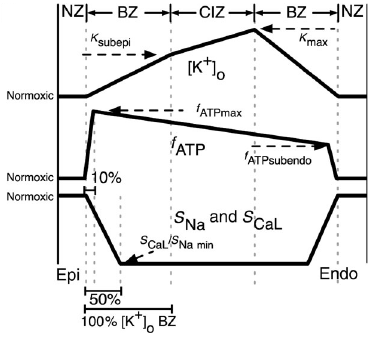
\includegraphics[width=0.5\textwidth]{spatial-ischaemia}
  \caption[Distribution of isch\ae{}mic properties in tissue.]{Distribution of hyperkal\ae{}mia, anoxia and acidosis in a transmural isch\ae{}mic tissue simulation. In non-transmural tissue, there is no gradient of \ko{} and $f$\sub{ATP} values within their respective isch\ae{}mic zones. This figure demonstrates the different ranges of border zones for the different components of isch\ae{}mia. Figure originally from \citet{Tice2007}.}
  \label{fig:spatial-ischaemia}
 \end{SCfigure}
 
 It should be remembered that the BZ is not a simple `buffer' between the CID and the NZ: Experimental data have also shown that a majority of extrasystoles occur in the peri-infarct zone, corresponding here with the BZ, \idest{} these data imply that the conditions in the BZ, and not just in the CID, promote arrhythmogenesis \citep{Chou2007}. This may be due in part to the difference in conditions between the CIZ and the NZ leading to a sharp heterogeneity present in the BZ, which then gives rise to arrhythmogenic conditions (more detail is given in \S\ref{subsubsec:alternans}). Furthermore, it has been shown that the heterogeneity within the BZ is not uniform, by which it is meant that the concentration gradients of different ions are not the same across the BZ \citep{Niederer2013}.
 
 However, it should be noted that changes during isch\ae{}mia are not limited to changes in the action potential---notable changes also occur in \cai{} and the contractile mechanisms of the cell (for a more detailed discussion of isch\ae{}mic changes in other ion concentrations, the reader is referred to \citet{Niederer2013}). Immediately post-occlusion, there is an increase in \cai{} until $\sim$2 min post-occlusion, followed by a decline (possibly to pre-occlusion levels), followed by a secondary increase at 5-15 min post-occlusion (see Fig.~\ref{fig:ca-ischaemia}) \citep{Lee1988, Mohabir1991, Camacho1993}. The increase in \cai{} can be describe more fully as
 \begin{itemize}
  \item Elevation of \casys{},
  \item Elevation of \cadia{},
  \item Broadening of systolic \ca{} peak (indicative of reduced SR uptake function),
  \item Increase in net amplitude of the \ca{} transient (though this is not always observed \citep{Camacho1993}).
 \end{itemize}
 Results indicate that the increase in \cai{} is due mostly to the effects of acidosis, but other mechanisms are required in addition to explain the initial increase \citep{Bers1982, Mohabir1991}. It has been hypothesised that the initial increase may be due to reduced SR uptake. The later increase may be augmented due to increased activation of \ica{} caused by the increase in $V$\sub{rest}, though \citet{Niederer2013} concluded that the increase in \cadia{} is due primarily to inhibition of \inak{}.
 
 The increase in \cai{} could be in small part be responsible for the increase in $V$\sub{rest} due to the action of \ca{}-activated cation channels \citep{Colquhoun1981}. The increase in \cai{} also occurs for low-flow isch\ae{}mia, \idest{} it is also likely to be present in the border zone to isch\ae{}mic tissue \citep{Camacho1993}.
 
 The secondary increase coincides with pH\sub{i} increasing to a `tipping point' at which changes in \cai{} are noted in purely acidic conditions, thus implying that this secondary increase is due entirely to decreasing pH\sub{i}.
 \begin{figure}
  \centering
  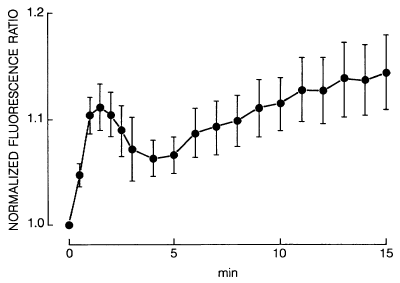
\includegraphics[width=0.8\textwidth]{ca-ischaemia}
  \caption[Effect of isch\ae{}mia on \cai{}.]{Mean systolic fluoresence ratio for rabbit hearts under isch\ae{}mic conditions, normalised to pre-isch\ae{}mic values. Data obtained using whole rabbit hearts loaded with indo-1, a cell-permeant fluorescent indicator for \ca{}, and demonstrate an initial increase in \cai{}, followed by a marginal decrease at 5-10 min post-occlusion, before increasing further. Figure originally from \citet{Mohabir1991}.}
  \label{fig:ca-ischaemia}
 \end{figure}
 
 There is a large body of evidence that the time constant of \cadia{} decline increases during isch\ae{}mia \citep{Allen1983, Camacho1994, Lee1988} (though not during hypoxia \citep{Silverman1991}). This may be achieved via a change in either \ca{} uptake to the SR, or via reduced extrusion of \ca{} via \inaca{}; evidence indicates that there is minimal change in \ca{}-uptake from the extracellular space during isch\ae{}mia \citep{Bourdillon1982}.
 
 For a fuller summary of the changes in SR function during isch\ae{}mia, both in terms of uptake (SERCA) and release (RyR), the reader is referred to \citet{Mubagwa1995}. Other details of changes in \ca{} handling during isch\ae{}mia are given in \citet{Talukder2009}. Note that possible changes in mitochondrial \ca{} handling are not considered in this thesis, as the consensus is that \ca{} pathophysiology is mainly due to changes in the SR \citep{Fauconnier2013}.
 
 Kinetic studies have demonstrated a decrease in action of SERCA with no change in \ca{} sensitivity, \idest{} there is a change in the number, not properties, of active SERCA. There is a large body of evidence for impaired SERCA action during isch\ae{}mia \citep{Dhalla1988, Temsah1999, Lee1967, Toba1978, Kaplan1992}. \citet{Krause1984} present results indicating SERCA becomes more sensitive to \cai{} as pH\sub{i} decreases, with a reduction in maximal velocity. However, while a decrease in maximal velocity was also seen in \citet{Kaplan1992}, there was no observed change in dissociation constant, representing \ca{} sensitivity. Antibody assays indicate a reduction in the number of active SERCA channels \citep{Levitsky1989}. As such, these results indicate that the conditions reduce the open probability of the SERCA channel. The reduction in SERCA action may be caused by ATP deficiency \citep{Camacho1993}, accompanied by other acidic effects \citep{Krause1984}. It has been suggested that free radicals are the means by which SERCA is impaired \citep{Temsah1999, Wang2013, Xu1997, Zweier1988}. The decrease in SERCA function persists after treatment for assays and the like, thus indicating that the causative agent in the change is not \cai{}, and the recovery of SERCA action after reperfusion indicates SERCA is not denatured. It is of note that results indicate that expression of SERCA and phospholamban are altered during cardiac remodelling post-infarct \citep{Sun2005}.
 
 It is unclear if release from the SR is also affected during isch\ae{}mia (increased loss would have a similar effect to reduced gain), with conflicting results. For example, \citet{Feher1989} used RyR blockers during isch\ae{}mia to achieve a reduction in rate of \ca{} uptake, indicating an influence of RyR in the process, and \citet{Fauconnier2011} demonstrated an increase SR leak (though this is likely a reperfusion effect). However, other results do not indicate a change in release \citep{Kaplan1992}, and others indicate RyR action is actually decreased (RyR channels are inhibited by NADH \citep{Wang2013}, which increases during isch\ae{}mia \citep{Esumi1991}).
 
 The r\^ole of \inaca{} during isch\ae{}mia is unclear---that it transiently reverses direction is not in doubt, but it is considered unlikely that this is a permanent feature of the isch\ae{}mic milieu \citep{Rodriguez2006}. \citet{Tani1989} demonstrated the decrease in pH led to an rapid initial increase in \nai{} (via the \H{}-\na{} exchanger), which then correlated with an increase in \cai{}, and \citet{Cross1998} demonstrated a correlation in male mice between increase \inaca{} and declined isch\ae{}mic recovery. Furthermore, inhibiton of \inaca{} has been shown to have cardioprotective properties. However, the reverse action of \inaca{} brings about the exact conditions required to return the exchanger to its normal operation, indicating that, at most, there is a reduction in \inaca{} during isch\ae{}mia. Such a hypothesis has been used computationally \citep{Pollard2002}, with peak \inaca{} reduced by $80\%$ for simulation of Phase 1B isch\ae{}mia.
 
 Opposing this increase in \cai{}, there is a counter-intuitive decrease in contractile strength of the myocyte \citep{Lee1988, Kaplan1992}, accompanied by an increase in diastolic tension \citep{Mubagwa1995}. There are many suggested mechanisms to explain this decline in contractile strength, despite the increase in \cai{}. \citet{Mohabir1991} postulated competitive inhibition by \H with \ca{} in the troponin-C complex \citep{Blanchard1984}, and thus the isch\ae{}mic decline in pH\sub{i} is responsible. Alternatively, \citet{Camacho1993} suggests the increase in inorganic phosphate (P\sub{i}) also attendant to isch\ae{}mia is responsible. However, against this fact is that contractile strength is reported to increase under hypoxic conditions \citep{Kihara1989}.
 
 Another way to explain the decrease in contractile strength is to appeal to the `garden hose effect', which is that the contractile strength of the myofilaments are reduced if the preceding relaxation is reduced \citep{Camacho1993, Kleber1987, Kleber1987b, Vogel1982} (though some findings dispute such a mechanism \emph{in vivo} \citep{Zhao1988}). As such, while an increase in \casys{} might indicate an increase in contractile strength, it is the increase in \cadia{}, preventing relaxation, that is more influential by this hypothesis. Of note for this hypothesis is the increase in the time constant for decline in left ventricular pressure \citep{Serizawa1981, Applegate1987, Serizawa1987, Isoyama1987}.
 
 At 2-3 min post-occlusion, \cai{} alternans develops. This is likely due to the function of the sarcoplasmic reticulum, rather than APD alternans: the smaller transient follows a higher diastolic \cai{}, indicating reduced SR release due to reduced SR sequestration. This is not to say that the SR release is impaired; rather it is a consequence of the steep-load relation of the SR previously mentioned \citep{Shiferaw2003, Restrepo2008}.
 
 Results from \citet{Coetzee1987} indicate that (mainly as a result of hypoxia), isch\ae{}mia reduces the incidence of DADs in guinea pigs, which would ordinarily be expected to increase in conditions of increased \cai{}.
 
 % Reperfusion also leads to an increase in Ca (Sharma1983) - due to alpha-adrenergic response (not sure if ischæmic or reperfusion-based, looks like latter), so application of alpha-adrenergic blocker can mitigate impact. This is unlikely due to mitigation of ischæmic damage.
 
 \subsubsection{Anoxia}
 \label{subsubsec:Anoxia}
 Anoxia represents the loss of oxygen from the isch\ae{}mic milieu, and is not directly modelled in most simulations, but is instead modelled by the effect on cellular respiration and the consequent decrease in ATP availability and increase of APD concentration. This change in ATP concentration is mainly felt through the activation of the \ikatp{} channel, which is the single greatest contributor to the shortening of the AP. This shortening of the AP, along with the increased inexcitability and shift of $V$\sub{rest}, works to protect the cell by avoiding excessive \K{} loss \citep{Carmeliet1999}.
 
 Two important different formulations of this channel have been developed: the first was originally by \citet{Ferrero1996}, and has been subsequently used by \citet{Trenor2007}, while the second was originally shown in \citet{Michailova2005}, and has been implemented in \citet{Terkildsen2007} and \citet{Michailova2007}. Both are dependent on both the ATP and ADP concentrations, and also \ko{}. The Ferrero implementation was used in a Luo-Rudy model, which can be considered as a general mammalian model, but much of its components are derived from guinea pig data. It includes dependency on the intracellular concentrations of \na{} and \mg{}. The Michailova model was originally implemented in a canine model, was subsequently adapted for a rabbit ventricular model, and lacks the sensitivity to \na{} and \mg{}. Both models are detailed in the appendix (\S\ref{sec:ikatp}).
 
 Activation of the \ikatp{} channels is achieved by decreasing [ATP]\sub{i} and increasing [ADP]\sub{i}. However, experimental data on the channel itself demonstrated that full activation of the channel in the cell would require a change in concentrations that are significantly greater than actually observed. It is thus currently thought that only minimal activation of the \ikatp{} channels is required to effect the changes in isch\ae{}mia; under this `spare channel' hypothesis \citep{Cook1988}, activation has been postulated as being $\sim0.8\%$ \citep{Rodriguez2002, Weiss1992, Ferrero1996, Trenor2007, Ferrero2003}. This small degree of activation allows for a very finely balanced activation of the channel to achieve the desired affect: consequently, it has been noted that the degree of activation of this channel is important for determining the vulnerability of the tissue/organ to reentry in regional isch\ae{}mia \citep{Ferrero2003a, Trenor2005}. However, within the isch\ae{}mic tissue, the activation of \ikatp{} is usually modelled as a linear increase of activation until it reaches maximum activation at 10 minutes post-occlusion \citep{Trenor2007, Tice2007}.
 
 \subsubsection{Hyperkal\ae{}mia}
 \label{subsubsec:hyperkalaemia}
 The onset of hyperkal\ae{}mia is known to follow a biphasic pattern: a rapid rise for the first $\sim10$ minutes of isch\ae{}mia, followed by a plateau phase (changes later in time are not discussed here). This rise is partly caused by the efflux of \K{} from the cell caused by activation of \ikatp{}, but this impact is negligible on its own---simulations have demonstrated that the increase requires the coordinated action of \ikatp{} with both inhibition of \inak{} and activation of an inward \na{}-pump, \inas{} \citep{Rodriguez2002}.
 
 The rate of increase, and final plateau level, of \ko{} has been shown to be rate-dependent, with values of \ko{} ranging from $12-17$ mM reached within $10-15$ min \citep{Rodriguez2002, Coetzee1987}. However, most simulation models take the time to plateau to be 10 min, and the plateau concentration to be $\sim12$ mM, though higher values have also been used in simulation \citep{Ferrero2003a, Trenor2007}. Research indicates that hyperkal\ae{}mia (with \ko{} greater than 12.5 mM) is vital to the development of reentry, with its absence precluding reentry \citep{Ferrero2003}.
 
 The hyperkal\ae{}mia is secondary to \ikatp{} in shortening the APD---its main effect is to affect the excitatory properties of the cell/tissue. For the first few minutes of isch\ae{}mia, the rise in \ko{} and its attendant rise in $V$\sub{rest} brings the cell closer to the activation threshold, and thus facilitates an increase in conduction velocity in tissue. However, once \ko{} rises beyond 8mM, the process of reactivation of \ina{} is inhibited by the increase in $V$\sub{rest}. This reduces the number of \ina{} channels available at the start of the AP, and this reduction in \ina{} magnitude is reflected in a reduction in the rate of depolarisation of the cell (a reduction in \dvdt{}); it has been shown that the recovery of \dvdt{} and the $h.j$ inactivation gates of \ina{} are similar \citep{Shaw1997}. In severe isch\ae{}mia (10-12 minutes after onset), this can lead to a biphasic upstroke \citep{Barrett1997}: the first phase corresponds to the reduced activation of \ina{}, and the second phase corresponds to the activation of \ica{} that completes the depolarisation. It should be noted that \dvdt{} is proportional as the square root to conduction velocity in tissue, so changes in cellular \dvdt{} correlates with changes in tissue restitution properties \citep{Kleber2004, Walton1983, Tasaki1957}---isch\ae{}mia is known to lead to a reduction in conduction velocity in tissue \citep{Caldwell2007}, though this is likely partly due to electrical uncoupling of the cells in isch\ae{}mic tissue \citep{Kleber1987}.
 
 The reduction in availability of \ina{} channels is also one of the main causative agents behind isch\ae{}mic \emph{post-repolarisation refractoriness} (PRR), and changes in myocardial excitability generally \citep{Coronel2012}.
 
 \subsubsection{Acidosis}
 \label{subsubsec:acidosis}
 The acidosis inherent in isch\ae{}mia is due mostly to the accumulation of \ce{CO2} that arises due to the cessation of blood flow, with a lesser r\^ole being played by the accumulation of lactate \citep{Ichihara1984}. The concentration of hydrogen ions that is represented by the pH is normally a tightly regulated feature of the cell, with small changes being responsible for major cellular dysfunction \citep{Chen1998}. During the first 10 minutes of isch\ae{}mia, intra- and extra-cellular pH drop linearly with time, with a $\sim1$ pH unit drop after 10 minutes \citep{Shaw1997, Neely1975, Mohabir1991}\footnote{It should be noted that the value of pH falls approximately linearly (see Fig.~10 in \citet{Mohabir1991}), and not the concentration of \H{}}.
 
 Prior work in computational modelling has shown the key importance of the impact this has on the ion flow through the \ina{} and \ica{} channels. It is postulated that acidosis is one of the key factors behind reduced uptake of \ca{} into the SR during isch\ae{}mia \citep{Krause1984}. The isch\ae{}mic pH drop reduces \ina{} maximum conductance by $25\%$ (as well as shifting its voltage-current dependence by $3.4$ mV) \citep{Kagiyama1982}. For guinea pig ventricular cells, a sigmoidal decrease in maximum conductance of \ica{} has been noted (with a $50\%$ reduction at pH $6.6$). In computational models of isch\ae{}mia, the effect of acidosis is thus modelled as a linear reduction in maximum conductance of \ina{} and \ica{} $\sim5$ minutes after the onset of isch\ae{}mia, until a $25\%$ reduction is reached after 10 minutes \citep{Trenor2007}; this corresponds to a pH of $\sim6.4$ \citep{Ferrero2003}. This, combined with the previously mentioned effects of hyperkal\ae{}mia, leads to a marked decrease in cell excitability and \dvdt{}, leading to a decrease in membrane exitability conduction velocity in tissue \citep{Shaw1997}.
 
 The isch\ae{}mic suppression of \inak{} \citep{Dhalla1988} has been shown to be due to acidosis, which linearly affects \inak{} \citep{Severi2002}.
 
 \subsection{Arrhythmogenesis}
 \label{subsec:arrhythmogenesis}
 One of the key reasons for studying isch\ae{}mia, as mentioned previously, is due to the cost of sudden cardiac death, and the r\^ole isch\ae{}mia plays in sudden cardiac death. As such, one of the key areas of research is how isch\ae{}mia can lead to sudden cardiac death, and thus the study of isch\ae{}mic arrhythmogenesis is vital.
 
 Studies have been conducted to establish the means by which isch\ae{}mic conditions can provide the substrate for arrhythmogenesis, and how it can lead to sustained arrhythmias. It should be emphasised at this point that arrhythmogenesis is not the preserve of isch\ae{}mia---arrhythmias can develop for any number of reasons, isch\ae{}mia being just one of them. It is of note that increasing susceptibility to arrhythmias is a consequence of something as harmless as aging, due to the increasing heterogeneity presented by certain breakdowns in the heart structure that occur naturally \citep{Spach1988}. Furthermore, it is not the case that tissue will `become' arrhythmic, and then, inevitably, arrhythmia will occur. Rather, tissue changes dynamically, and while it may have greater arrhythmogenic properties, this does not necessarily guarantee arrhythmia \citep{Weiss2006}.
 
 Fibrillation in ventricular tissue can be initiated and maintained by several different mechanisms, including:
 \begin{itemize}
  \item Ectopic beats \citep{Haissaguerre1998, Tobon2010, Zhang2011};
  \item Spiral/scroll waves and rotors \citep{Jalife2003, Jalife2009, Pandit2013};
  \item Stable points of reentry \citep{Mandapati2000, Allessie1977};
  \item Unidirectional block \citep{Allessie1976, Gough1985};
  \item Vortex formation \citep{Cabo1996}.
 \end{itemize}
 Isch\ae{}mia has been shown to provide the substrate for all of these mechanisms. Furthermore, research has demonstrated that structural heterogeneities, another potential side-effect of isch\ae{}mia, can increase incidence of arrhythmia and other atypical electrical activity, \eg{} early after-depolarisations (EADs) \citep{Auerbach2011}.
 
 This increase in \emph{dispersion} of electrophysiological properties is a key area for investigation for its arrhythmogenic properties \citep{Kuo1983}. Recently, there has been increased awareness of the importance of multiple different factors simulataneously for the development of arrhythmias in isch\ae{}mic tissue. While isch\ae{}mia is well known to increase the vulnerability to ectopic beats \citep{Zhang2011}, the `width' of the vulnerability window (the range of coupling intervals at which an ectopic beat will lead to sustained arrhythmias) does not increase throughout the onset of isch\ae{}mia, \idest{} arrhythmogenic risk does not increase linearly with duration of isch\ae{}mia \citep{Tice2007, Romero2009a, Barrett1997}. Furthermore, the properties of the tissue play a profound r\^ole in arrhythmogenesis. For example, it is insufficient to only have unidirectional block in tissue for a sustained arrhythmia: an interaction between the coupling interval, the unidirectional block, the restitution properties of the tissue, the scale of the block, and the conduction velocity in the tissue are all required \citep{Coronel2009, Cherry2012}. As a consequence, there is a minimum size of tissue for which arrhythmias can be maintained, though this size can vary depending on the circumstances of the tissue \citep{Adeniran2011}. This is not to say that increased dispersion, evident on the cellular scale, is meaningless---quite the opposite. Rather, the dispersion can provide the underlying properties that, given the correct interaction, leads to dangerous tissue properties.
 
 As has previously been noted, the cardiac system is an inherently dynamic one---multiple different currents interact in a time- and voltage-dependent manner with each other, and other complicating factors, to produce the complete AP and associated cardiac contraction. These interactions vary depending on the condition of the heart, and the environment the heart is found in. This dynamic nature is true not only for the normal, `healthy' conditions, but also for the pathological conditions such as arrhythmia and isch\ae{}mia. As such, with the consideration that the key thrust of this thesis is concerned with variability in ion channel properties and its correlation with experimentally observed variation, it is necessary to consider the ionic bases that exist for arrhythmias, and how these manifest in arrhythmia.
 
 What follows is a brief summary of some pertinent ion channel mutations, their possible effects, and how these electrical alterations can lead to arrhythmia; I do not pretend to present a comprehensive compilation of the possible mutations, for the simple fact that they are legion, and it is beyond the remit of this thesis to discuss them.
 
 \subsubsection{Delayed After Depolarisations}
 \label{subsubsec:dad}
 Delayed after depolarisations (DADs) refer to a spontaneous depolarisation of the cell after cellular repolarisation with no external stimulus. Along with early after depolarisations (see next section), thesecan provide the source for ectopic beats, which lead to reentry. DAD frequency is sensitive to increases in \cai{}. The underlying mechanism by which the \cai{} overload can occur is usually attributed to changes in \ica{}, but can also be due to alterations in CICR (a mechanism which can also result in EADs) \citep{Volders1997}. Due to the increased \cai{}, this activates \inaca{}, which due to its electrogenic properties, depolarises the cell, causing a DAD \citep{Clusin2003}.
 
 The occurence of DADs is reduced during isch\ae{}mia (though not in the border zone or otherwise partly isch\ae{}mic tissue), mostly due to the action of hypoxia, but DAD amplitude increases after reperfusion of the isch\ae{}mic tissue \citep{Coetzee1987, Ferrier1985}.
 
 \subsubsection{Early After Depolarisations}
 \label{subsubsec:ead}
 Early after depolarisations (EADs) occur before cellular repolarisation, and usually occurs under situations when the AP is prolonged. There are many possible ionic causes for EADs: the most commonly muted ionic bases for EADs are changes in \ica{} and \ina{}: \ina{} mutations resulting in reduced inactivation work to prolong the action potential \citep{Clancy2005, Hashambhoy2011, Hiraoka1992}. If the \ca{} concentration near the sarcolemmal surface remains high during the AP, an EAD may also be initiated by \inaca{ } \citep{Volders1997}. The upstroke of an EAD is often slower than the usual AP upstroke, due to the fact that it is based on \ica{}, rather than \ina{} (the lack of repolarisation means the \ina{} current is still deactivated) \citep{Clusin2003}.
 
 There are clinical similarities between EADs and the presentation of LQTS, but the r\^ole has not been confirmed \citep{Clusin2003}.
 
 \subsubsection{Alternans}
 \label{subsubsec:alternans}
 % Need to rewrite this to make it more coherent - currently jumps all over the place
 Alternans is a phenomenon wherein the AP or \cai{} alternate properties from beat to bear. Usually (and for the majority of the following discussion), this is defined in terms of the duration of the AP alternating between long/short duration and the  \cai{} transient alternating between large/small magnitude, respectively. However, it should be remembered that alternans of the AP amplitude also exists, and may reflect the inability of \ina{} to fully recover between beats. Such a process could lead to a reduction in plateau amplitude, which in turn could lead to \cai{} alternans \citep{Clusin2003}. AP amplitude and APD alternans are not exclusive of each other.
 
 In tissue, alternans can be either spatially concordant or spatially discordant (Fig.~\ref{fig:alternans}). \citet{Qian2001} demonstrated that \ca{} alternans `self-organises' into regions of tissue with the same phase, and hypothesised that this was due to movement of \ca{} across gap junctions to neighbouring cells allowed some degree of synchronisation.
 \begin{SCfigure}
  \centering
  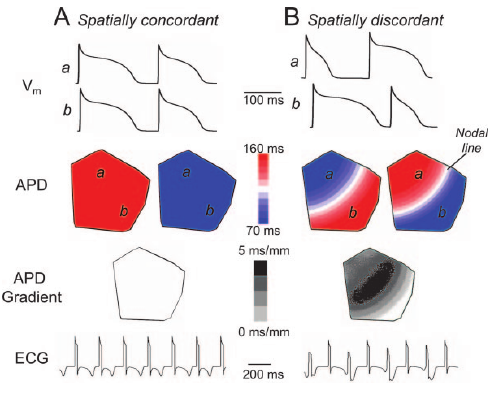
\includegraphics[width=0.5\textwidth]{alternans}
  \caption[Spatially cordant and spatially discordant alternans in cardiac tissue]{Spatially cordant (left column, A) and spatially discordant (right column, B) alternans in cardiac tissue. The top panel shows the AP and \cai{} data for two separate locations in the tissue. The second panel shows the APD during each beat, with the third panel showing the APD gradient resulting from such distributions. The bottom panel shows the simulated ECG for each tissue. These simulations were performed using a modified Luo-Rudy model from \citet{Qu2000}. Figure originally from \citet{Weiss2006}.}
  \label{fig:alternans}
 \end{SCfigure}
 
 It is a consequence of spatially discordant alternans that, between the out-of-phase regions there is a region where no alternans is present (referred to as the \emph{nodal line}). It is this region that, due to the APD/\cai{} gradients being steepest here, is most predisposed to develop unidirectional conduction block---a region with long APD remains inexcitable when a region with short APD is excited, with the resulting AP being blocked initially, forming a reentrant circuit \citep{Laurita2008}. As concordant alternans does not demonstrate this dispersion of properties, it is less arrhythmogenic than discordant alternans. It has been shown that heterogeneity is not required for spatially discordant alternans to occur---due to the dependence of conduction velocity on diastolic interval (conduction velocity restitution), rapid pacing can induce spatially discordant alternans in homogeneous tissue \citep{Watanabe2001}. It should be noted that the isch\ae{}mic reduction in \ina{} availability increases the DI range over which CV varies, and thus increases the risk of this phenomenon. Ectopic beats have also been shown to induce spatially discordant alternans in homogeneous tissue.
 
 There is no firm evidence as to whether APD alternans drives \ca{} alternans or vice versa, but mounting evidence indicates the latter to be the case. Evidence for this is varied. \citet{Lee1988} demonstrated that, when APD alternans and \ca{} alternans were both present (and recorded simultaneously), there was no variation in the APD until after the \ca{} transient had reached its peak---it was only after this that the APD alternans manifested. \citet{Chudin1999} were able to induce \ca{} alternans without APD alternans at rapid pacing rates in cell (demonstrating an instability in the \ca{} system independent of the AP). Similar results have been achieved \emph{in vivo} \citep{Aistrup2006} and \emph{in silico} \citep{Sato2006}.
 
 Research is ongoing to determine the mechanisms behind \ca{} alternans. A simple hypothesis is that, at rapid pacing rates, there is simply not enough time for the SR to resequester the \ca{} it has previously expended. Thus, the subsequent \ca{} release from the SR is smaller, leaving more time for a complete resequestration of the \ca{} by the SR. Mechanistically, \citet{Shiferaw2003} were able to reproduce \ca{} alternans at rapid pacing rate without APD alternans by including a steep release-load relation for the \ca{} sequestered in the SR. On a molecular level, evidence indicates that alternans prone regions express significantly less SERCA2a and RyR---this indicates responsibility lies with both SR uptake and release. Research is ongoing to find methods to protect these functions in isch\ae{}mia/reperfusion therapy \citep{Wang2013}.
 
 The coupling between APD and \ca{} alternans can be either positive or negative, \idest{} a long APD corresponds with a large \cai{} transient, or with a small \cai{} transient. Which of these relations predominates depends on the dominant current---a large \cai{} transient enhances both \iks{} and inactivation of \ica{} (which would shorten the APD, \idest{} negative coupling), but this process also enhances the activity of the exchanger \inaca{} (which would prolong the APD, \idest{} positive coupling) \citep{Shiferaw2005}. Whether postive or negative coupling predominates suggests which mechanism is the primary. Positive coupling is the more common of the two \citep{Laurita2008}, but negative coupling has been noted in isch\ae{}mia \citep{Lee1988}.
 
 The question can be asked: is it APD alternans that leads to \ca{} alternans, or vice versa? Mounting experimental evidence indicates that the onset of APD alternans is caused by instability in the cellular \cai{} dynamics, rather than by a steep APD restitution curve \citep{Goldhaber2005, Pruvot2004}. There are also expected spatial differences in the nodal line distributions depending on whether the alternans are AP or \ca{} driven \citep{Weiss2006}.
 
 while the restitution curve can provide a useful indication of when tissue is at risk of developing alternans (when the gradient is greater than 1), it must be remembered that this assumes that the APD depends entirely on the preceding DI---this is not the case. It has been observed that alternans can occur when the restitution curve is flat, and no alternans when it is steep \citep{Shiferaw2005}. Part of the reason for these anomalies is the influence of \cai{}. It is of note that isch\ae{}mia has been observed to flatten the restitution curve \citep{Taggart1996} while the occurence of alternans is increased \citep{Qian2001}. Much work has been conducted to try and determine the mechanisms behind \ca{} alternans \citep{Shiferaw2003, Weiss2006}.
 
 \subsubsection{Spiral Waves \& Rotors}
 \label{subsubsec:spiralWaves-rotors}
 Spiral/scroll waves and rotors are a key area of research in arrhythmias, and consist of a curved wavefront and curved wavetail that meet each other at a `phase singularity' \citep{Fitzhugh1960, Fitzhugh1961, Gray1998}. This singularity processes around an excitable core, with this core able to be either stationary or mobile. Not only do spiral waves represent a local source of activation within ventricular tissue, they are also liable to break-up, leading to fibrillation \citep{Riccio1999}.
 
 Of the previously discussed ion channels, three are known to have an effect on rotor dynamics: \ina{}, \ikix{} and \iks{}. Block of \ica{} has been shown to stabilise reentry, but its exact r\^ole is still unclear \citep{Jalife2003, Jalife2009}. \ina{} is of note due to its impact on the conduction velocity of the AP, and thus affects the speed (and thus dominant frequency) of the spiral wave. Reducing \ina{} also increases the meander of the core of the rotor. \ikix{} mediates the electrotonic interactions between the unexcited core and the immediate surroundings. It also stabilises reentry due to its ability to shorten APD and reduce conduction velocity near the core, thus preventing wavefront-wavetail interactions that could destabilise and breakup the rotor. Furthermore, by decreasing the resting membrane potential, it facilitates the reactivation of \ina{} \citep{Pandit2013}. \ikr{} has been shown to accelerate the rotor, but not to a degree comparable to the effect of \ikix{}. While \iks{} does not in itself change the rotor dynamics, it is important in determining post-repolarisation refactoriness and wave break formation, and thus important for the transition from tachycardia to fibrillation. It is also interesting to note that regional cooling of a rotor decreases its frequency and increases the rotor's meander, causing it to collide with a boundary and extinguish \citep{Yamazaki2012}.
 
 \subsubsection{Re-entry}
 \label{subsubsec:reentry}
 Generally speaking, \emph{re-entry} refers to the mechanism by which the electrical activity of the heart does not complete its `normal' circuit, but instead enters a process whereby it self-excites itself (hence the term)---the process has also been termed `circus movement'. Such a process can occur in many forms, as spiral waves (\S\ref{subsubsec:spiralWaves-rotors}) or figure-of-eight patterns \citep{Ferrero2003} to name but two. Modes of re-entry are often associated with tachycardia, and can subsequently lead to fibrillation and other forms of arrhythmogenesis.
 
 It must be noted that ectopic beats are not required to initiate reentry---dispersion of electric properties in the tissue are sufficient. An example is the case where there are two regions with different effective refactory periods (ERPs), one of which is greater than the CL, the other where it is less. The region with ERP > CL is thus unexcitable when the wavefront is incident, and conduction block occurs at this region. However, the region with ERP < CL is excitable, and thus the wavefront progresses through this region, and subsequently may excite the previously blocked region in a figure-of-eight reentry pattern \citep{Weiss2006}.

 \biblio
\end{document}
